% Options for packages loaded elsewhere
% Options for packages loaded elsewhere
\PassOptionsToPackage{unicode}{hyperref}
\PassOptionsToPackage{hyphens}{url}
\PassOptionsToPackage{dvipsnames,svgnames,x11names}{xcolor}
%
\documentclass[
  letterpaper,
  DIV=11,
  numbers=noendperiod]{scrartcl}
\usepackage{xcolor}
\usepackage{amsmath,amssymb}
\setcounter{secnumdepth}{5}
\usepackage{iftex}
\ifPDFTeX
  \usepackage[T1]{fontenc}
  \usepackage[utf8]{inputenc}
  \usepackage{textcomp} % provide euro and other symbols
\else % if luatex or xetex
  \usepackage{unicode-math} % this also loads fontspec
  \defaultfontfeatures{Scale=MatchLowercase}
  \defaultfontfeatures[\rmfamily]{Ligatures=TeX,Scale=1}
\fi
\usepackage{lmodern}
\ifPDFTeX\else
  % xetex/luatex font selection
\fi
% Use upquote if available, for straight quotes in verbatim environments
\IfFileExists{upquote.sty}{\usepackage{upquote}}{}
\IfFileExists{microtype.sty}{% use microtype if available
  \usepackage[]{microtype}
  \UseMicrotypeSet[protrusion]{basicmath} % disable protrusion for tt fonts
}{}
\makeatletter
\@ifundefined{KOMAClassName}{% if non-KOMA class
  \IfFileExists{parskip.sty}{%
    \usepackage{parskip}
  }{% else
    \setlength{\parindent}{0pt}
    \setlength{\parskip}{6pt plus 2pt minus 1pt}}
}{% if KOMA class
  \KOMAoptions{parskip=half}}
\makeatother
% Make \paragraph and \subparagraph free-standing
\makeatletter
\ifx\paragraph\undefined\else
  \let\oldparagraph\paragraph
  \renewcommand{\paragraph}{
    \@ifstar
      \xxxParagraphStar
      \xxxParagraphNoStar
  }
  \newcommand{\xxxParagraphStar}[1]{\oldparagraph*{#1}\mbox{}}
  \newcommand{\xxxParagraphNoStar}[1]{\oldparagraph{#1}\mbox{}}
\fi
\ifx\subparagraph\undefined\else
  \let\oldsubparagraph\subparagraph
  \renewcommand{\subparagraph}{
    \@ifstar
      \xxxSubParagraphStar
      \xxxSubParagraphNoStar
  }
  \newcommand{\xxxSubParagraphStar}[1]{\oldsubparagraph*{#1}\mbox{}}
  \newcommand{\xxxSubParagraphNoStar}[1]{\oldsubparagraph{#1}\mbox{}}
\fi
\makeatother


\usepackage{longtable,booktabs,array}
\newcounter{none} % for unnumbered tables
\usepackage{calc} % for calculating minipage widths
% Correct order of tables after \paragraph or \subparagraph
\usepackage{etoolbox}
\makeatletter
\patchcmd\longtable{\par}{\if@noskipsec\mbox{}\fi\par}{}{}
\makeatother
% Allow footnotes in longtable head/foot
\IfFileExists{footnotehyper.sty}{\usepackage{footnotehyper}}{\usepackage{footnote}}
\makesavenoteenv{longtable}
\usepackage{graphicx}
\makeatletter
\newsavebox\pandoc@box
\newcommand*\pandocbounded[1]{% scales image to fit in text height/width
  \sbox\pandoc@box{#1}%
  \Gscale@div\@tempa{\textheight}{\dimexpr\ht\pandoc@box+\dp\pandoc@box\relax}%
  \Gscale@div\@tempb{\linewidth}{\wd\pandoc@box}%
  \ifdim\@tempb\p@<\@tempa\p@\let\@tempa\@tempb\fi% select the smaller of both
  \ifdim\@tempa\p@<\p@\scalebox{\@tempa}{\usebox\pandoc@box}%
  \else\usebox{\pandoc@box}%
  \fi%
}
% Set default figure placement to htbp
\def\fps@figure{htbp}
\makeatother


% definitions for citeproc citations
\NewDocumentCommand\citeproctext{}{}
\NewDocumentCommand\citeproc{mm}{%
  \begingroup\def\citeproctext{#2}\cite{#1}\endgroup}
\makeatletter
 % allow citations to break across lines
 \let\@cite@ofmt\@firstofone
 % avoid brackets around text for \cite:
 \def\@biblabel#1{}
 \def\@cite#1#2{{#1\if@tempswa , #2\fi}}
\makeatother
\newlength{\cslhangindent}
\setlength{\cslhangindent}{1.5em}
\newlength{\csllabelwidth}
\setlength{\csllabelwidth}{3em}
\newenvironment{CSLReferences}[2] % #1 hanging-indent, #2 entry-spacing
 {\begin{list}{}{%
  \setlength{\itemindent}{0pt}
  \setlength{\leftmargin}{0pt}
  \setlength{\parsep}{0pt}
  % turn on hanging indent if param 1 is 1
  \ifodd #1
   \setlength{\leftmargin}{\cslhangindent}
   \setlength{\itemindent}{-1\cslhangindent}
  \fi
  % set entry spacing
  \setlength{\itemsep}{#2\baselineskip}}}
 {\end{list}}
\usepackage{calc}
\newcommand{\CSLBlock}[1]{\hfill\break\parbox[t]{\linewidth}{\strut\ignorespaces#1\strut}}
\newcommand{\CSLLeftMargin}[1]{\parbox[t]{\csllabelwidth}{\strut#1\strut}}
\newcommand{\CSLRightInline}[1]{\parbox[t]{\linewidth - \csllabelwidth}{\strut#1\strut}}
\newcommand{\CSLIndent}[1]{\hspace{\cslhangindent}#1}



\setlength{\emergencystretch}{3em} % prevent overfull lines

\providecommand{\tightlist}{%
  \setlength{\itemsep}{0pt}\setlength{\parskip}{0pt}}



 


\usepackage{booktabs}
\usepackage{caption}
\usepackage{longtable}
\usepackage{colortbl}
\usepackage{array}
\usepackage{anyfontsize}
\usepackage{multirow}
\KOMAoption{captions}{tableheading}
\makeatletter
\@ifpackageloaded{tcolorbox}{}{\usepackage[skins,breakable]{tcolorbox}}
\@ifpackageloaded{fontawesome5}{}{\usepackage{fontawesome5}}
\definecolor{quarto-callout-color}{HTML}{909090}
\definecolor{quarto-callout-note-color}{HTML}{0758E5}
\definecolor{quarto-callout-important-color}{HTML}{CC1914}
\definecolor{quarto-callout-warning-color}{HTML}{EB9113}
\definecolor{quarto-callout-tip-color}{HTML}{00A047}
\definecolor{quarto-callout-caution-color}{HTML}{FC5300}
\definecolor{quarto-callout-color-frame}{HTML}{acacac}
\definecolor{quarto-callout-note-color-frame}{HTML}{4582ec}
\definecolor{quarto-callout-important-color-frame}{HTML}{d9534f}
\definecolor{quarto-callout-warning-color-frame}{HTML}{f0ad4e}
\definecolor{quarto-callout-tip-color-frame}{HTML}{02b875}
\definecolor{quarto-callout-caution-color-frame}{HTML}{fd7e14}
\makeatother
\makeatletter
\@ifpackageloaded{caption}{}{\usepackage{caption}}
\AtBeginDocument{%
\ifdefined\contentsname
  \renewcommand*\contentsname{Table of contents}
\else
  \newcommand\contentsname{Table of contents}
\fi
\ifdefined\listfigurename
  \renewcommand*\listfigurename{List of Figures}
\else
  \newcommand\listfigurename{List of Figures}
\fi
\ifdefined\listtablename
  \renewcommand*\listtablename{List of Tables}
\else
  \newcommand\listtablename{List of Tables}
\fi
\ifdefined\figurename
  \renewcommand*\figurename{Figure}
\else
  \newcommand\figurename{Figure}
\fi
\ifdefined\tablename
  \renewcommand*\tablename{Table}
\else
  \newcommand\tablename{Table}
\fi
}
\@ifpackageloaded{float}{}{\usepackage{float}}
\floatstyle{ruled}
\@ifundefined{c@chapter}{\newfloat{codelisting}{h}{lop}}{\newfloat{codelisting}{h}{lop}[chapter]}
\floatname{codelisting}{Listing}
\newcommand*\listoflistings{\listof{codelisting}{List of Listings}}
\makeatother
\makeatletter
\makeatother
\makeatletter
\@ifpackageloaded{caption}{}{\usepackage{caption}}
\@ifpackageloaded{subcaption}{}{\usepackage{subcaption}}
\makeatother
\usepackage{bookmark}
\IfFileExists{xurl.sty}{\usepackage{xurl}}{} % add URL line breaks if available
\urlstyle{same}
\hypersetup{
  pdftitle={Everyone Watches Women's Basketball: Attendance and Fan Engagement in the WNBA},
  pdfauthor={Gabriela Eastwood; Benjamin S. Baumer; Andrew Zimbalist},
  pdfkeywords={WNBA, Game Attendance},
  colorlinks=true,
  linkcolor={blue},
  filecolor={Maroon},
  citecolor={Blue},
  urlcolor={Blue},
  pdfcreator={LaTeX via pandoc}}


\title{Everyone Watches Women's Basketball: Attendance and Fan
Engagement in the WNBA}
\author{Gabriela Eastwood \and Benjamin S. Baumer \and Andrew Zimbalist}
\date{2026-07-06}
\begin{document}
\maketitle
\begin{abstract}
We examine how the relationships between attendance and three notions of
fan engagement have changed over the history of the WNBA. Previous
research suggests that stronger professional sports teams draw higher
live game attendance. However, there is ongoing doubt about the extent
to which that relationship holds in the WNBA. We improve upon previous
research by modeling attendance in the broader context of the league's
growth from 1997-2025, and find that the factors that drive fan demand
have evolved as the league has matured. We test whether three leading
theories of fan behavior---quality of play, loss aversion, and outcome
uncertainty---have become more important drivers of attendance as the
league has grown. We use game-level attendance data reported directly by
the WNBA as well as team Elo ratings and game-by-game home win
probabilities and find that in recent years fans are increasingly likely
to attend games in response to quality of play and loss aversion
factors. We also find strong support for the large impact of Indiana
Fever guard Caitlin Clark's presence upon attendance. Our results
suggest that the WNBA is entering a new era in which fans are choosing
to attend games to watch good basketball rather than novelty-driven
interest or broader support for women's sports. This, in turn, is
consistent with a more durable popularity for the league.
\end{abstract}


\section{Introduction}\label{sec-intro}

In the years prior to the 2020 WNBA collective bargaining agreement
(CBA), NBA Commissioner Adam Silver publicly characterized the women's
league as unpopular and unprofitable (Garcia 2020). Again during the CBA
renegotiations in 2025, NBA and WNBA leadership made similar negative
claims about the women's league's long term viability. While leadership
has been ironically pessimistic about the health of the WNBA in recent
years, their claims stand in tension with recent trends: the league has
enjoyed a significant increase in attendance and fan interest in the
past several seasons.

While this trend is encouraging for anyone interested in the success of
the WNBA, further breaking down the underlying components of this trend
is necessary both to explain and sustain this growth. For decades,
league officials and sports economists have debated the primary drivers
of game attendance, identifying game-related and market-related factors
impacting fan interest and game attendance. Much of this research,
beginning with foundational work in the 1970s, assumes that fans are
more likely to attend games when the home team is expected to do well.
This relationship is widely tested and supported in men's professional
sports, but women's leagues and the WNBA in particular are still largely
underresearched. As a relatively young league with rapid growth in
viewership (WNBA 2024) but limited publicly available financial data,
game attendance remains the most readily available proxy for public
interest in the WNBA. In this paper we set out to determine how the
underlying causes shape game attendance and explain these more recent
trends. Specifically, we focus on whether on-court factors are becoming
more important to WNBA game attendance in recent years.

\subsection{Existing scholarship on team performance and game
attendance}\label{existing-scholarship-on-team-performance-and-game-attendance}

A key line of research in sports economics links fan demand to
expectations about game outcomes. Early work such as the
uncertainty-of-outcome hypothesis suggests that attendance is higher
when game results are less predictable, increasing perceived excitement.

\begin{tcolorbox}[enhanced jigsaw, arc=.35mm, bottomrule=.15mm, bottomtitle=1mm, breakable, colback=white, colbacktitle=quarto-callout-note-color!10!white, colframe=quarto-callout-note-color-frame, coltitle=black, left=2mm, leftrule=.75mm, opacityback=0, opacitybacktitle=0.6, rightrule=.15mm, title=\textcolor{quarto-callout-note-color}{\faInfo}\hspace{0.5em}{Ben}, titlerule=0mm, toprule=.15mm, toptitle=1mm]

We need a citation for the Uncertainty of Outcome Hypothesis

\end{tcolorbox}

Coates et al. (2014) use more recent behavioral economics models to
suggest that people evaluate gains and losses relative to a reference
point and tend to dislike losses more than they like equivalent wins.
They argue that applying this idea of loss aversion may better explain
why fans choose to go to games than the uncertainty of outcome
hypothesis. They use MLB live-game attendance data to find patterns
consistent with the hypothesis that fans are less likely to attend games
in which they expect the home team to lose (Coates et al. 2014). These
frameworks together suggest that attendance decisions are sensitive not
only to team quality, but to expectations about competitive performance
and likely game outcomes.

\begin{tcolorbox}[enhanced jigsaw, arc=.35mm, bottomrule=.15mm, bottomtitle=1mm, breakable, colback=white, colbacktitle=quarto-callout-note-color!10!white, colframe=quarto-callout-note-color-frame, coltitle=black, left=2mm, leftrule=.75mm, opacityback=0, opacitybacktitle=0.6, rightrule=.15mm, title=\textcolor{quarto-callout-note-color}{\faInfo}\hspace{0.5em}{Ben}, titlerule=0mm, toprule=.15mm, toptitle=1mm]

Let's say more about expected utility and non-linearity

\end{tcolorbox}

In the first study in sports economics that sought to empirically
identify the factors that affected attendance, Noll (1974) considered
data from MLB, the NFL, NHL, NBA and ABA (American Basketball
Association) for the 1969-70 and 1970-71 seasons and found that demand
was a function of population, interactions of income with star players,
team win percentage, and per capita income. Multiple subsequent studies
on men's professional team sports continued to find a statistically
significant correlation between team quality and attendance. Differences
in the literature over how to measure team quality (wins, wins lagged,
number of championships in past years, win probability, star power),
attendance (logs, lags, linear regression or censored), the inclusion of
control variables and non-linear forms also emerged (Wiseman and
Chatterjee 2003; Woltring 2018; Kim and Chang 2023; DeSchriver and
Jensen 2002; Paul et al. 2019).

Studies of attendance and winning percentage often consider the latter
as causing the former. Davis (2008) and Horowitz (2007) both found that
attendance and winning percentage were related. Horowitz concluded a
bidirectional relationship between the two, while Davis suggested that
causation runs from winning percentage to attendance. In a following
study, Davis (2009) found winning percentage as a significant
determinant of attendance for 12 National League teams. The study did
not establish causation both ways. Lemke et al. (2010) found attendance
increases as home team win probability increases. There is evidence that
causation may run from attendance to winning percentage, but the bulk of
the literature has found the other way.

\begin{tcolorbox}[enhanced jigsaw, arc=.35mm, bottomrule=.15mm, bottomtitle=1mm, breakable, colback=white, colbacktitle=quarto-callout-note-color!10!white, colframe=quarto-callout-note-color-frame, coltitle=black, left=2mm, leftrule=.75mm, opacityback=0, opacitybacktitle=0.6, rightrule=.15mm, title=\textcolor{quarto-callout-note-color}{\faInfo}\hspace{0.5em}{Ben}, titlerule=0mm, toprule=.15mm, toptitle=1mm]

What evidence? We should cite something if there is evidence.

Also, really? Attedance causes winning percentage to rise???

\end{tcolorbox}

Finally, situating these revenue models within the broader league
structure, sports economists have written extensively about the
relationship between winningness and team revenue, particularly about
how competitive balance benefits teams across the league in generating
revenue.

\begin{tcolorbox}[enhanced jigsaw, arc=.35mm, bottomrule=.15mm, bottomtitle=1mm, breakable, colback=white, colbacktitle=quarto-callout-note-color!10!white, colframe=quarto-callout-note-color-frame, coltitle=black, left=2mm, leftrule=.75mm, opacityback=0, opacitybacktitle=0.6, rightrule=.15mm, title=\textcolor{quarto-callout-note-color}{\faInfo}\hspace{0.5em}{Ben}, titlerule=0mm, toprule=.15mm, toptitle=1mm]

What revenue models??

\end{tcolorbox}

While teams and fans want to win as many games as possible, significant
imbalance in winning percentages across a professional sports league
will tend to decrease viewership as spectators will only watch a game if
they have some uncertainty about the outcome (Perline et al. 2018). In
NCAA basketball, Perline et al. (2018) examine the standard deviation
and the range of winning percentages for teams in the women's Division I
and determine that the women's game is significantly less balanced than
the men's game. They hypothesize that the difference in the competitive
balance of the men's and women's games could be one cause of lower
revenue generation and attendance in the women's game.

\subsection{Why is the WNBA different?}\label{why-is-the-wnba-different}

Agha and Berri (2023) argue that a major reason why attendance is
considerably lower at WNBA games relative to NBA games is that the
women's league is still in its early years, only beginning play in 1997
compared to the NBA's 1946. To account for this, they compare attendance
in the tenth season of the WNBA (2006) and the NBA (1955/56) (p.~36). In
their respective tenth years, the WNBA average attendance per home game
exceeded the NBA's by more than 2,000 fans per game. They do not control
for the growth in population over the period 1955-2006. This comparison
suggests that the current disparity in attendance between the women's
and men's league should not be interpreted simply as a lack of demand,
but rather a sign of the league's maturity. Considering the league's age
as a factor in demand for attendance, we inquire further into whether
patterns of fan behavior change as the league matures. Agha and Berri
(2023) attempt to establish whether different forces shape demand for
attendance in the WNBA and the NBA, finding that team performance was
not a statistically significant predictor of game attendance in the
WNBA. As noted above, this is contrary to the virtually unanimous
finding in the existing scholarship for men's leagues. However, their
study only employed data from 2004 through 2017 and thus cannot capture
the more recent improvements in attendance shown in
Figure~\ref{fig-boxplots}. They also measure a team's strength using the
team's winning percentage from the previous year which raises issues
because fans are more likely to respond to the more recent performance
of the team. Thus, while a team's win percentage in 2016 might have an
appreciable impact on the team's attendance at the beginning of the 2017
season, as the season wears on, this impact should diminish.

The disparity between raw attendance numbers and attendance driving
factors in the NBA and WNBA cannot be attributed to the age of the
leagues alone. Additional important factors include: the WNBA plays
during the summer months in order to promote arena use outside of the
NBA season; there is less money spent on promotion; reduced media
coverage; historical prejudice; poorer arena amenities and age, among
others.

Sport management literature also includes several studies that find a
major motivation behind fandom for women's sports leagues to be an
area's overall support for feminist issues, suggesting that fans in
those areas may attend games out of political support rather than to see
good basketball (Delia 2020; Guest and Luijten 2018; Leslie-Walker and
Mulvenna 2022). Factors like the summer season, reduced media coverage,
and the association of game attendance with feminist causes all
contribute to the argument that the WNBA functions fundamentally
differently to the NBA---at least in terms of attendance drivers. This
conception of the WNBA as fundamentally different from the NBA is
dangerous both to the league's reputation and future growth, motivating
our more thorough examination of game attendance in the context of the
league's history.

\subsection{Our contribution}\label{our-contribution}

It is reasonable to anticipate that as women's sports mature and are
perceived increasingly as a normal sports league (rather than a
political concession or oddity) they will begin to assert similar fan
demand characteristics. In particular, fan demand should become more
responsive to team quality. Using game attendance and team performance
data from 1997 through 2025, we test these hypotheses. In viewing more
recent attendance figures for the WNBA in the context of the league's
history, we determine whether predictors of attendance have shifted over
time. Specifically, we find that in recent years the strength of the
effect of a game's uncertainty, the strength of both teams, and the
likelihood of a home team win, on game attendance has increased,
paralleling documented trends in men's leagues.

\section{Data}\label{sec-data}

\subsection{Game logs}\label{game-logs}

Our analysis is based on game-level data that spans WNBA history,
beginning in 1997 and continuing through the end of the 2025 season. Our
final data set contains observations from 6,164 games.

First, we collected game-level attendance data from (Zimmerman 2026), an
online repository for women's basketball data that collects attendance
numbers directly from the league's records\footnote{Note that, as in
  most sports leagues, there is always the possibility of finagling with
  game attendance figures. The WNBA appears to give attendance counting
  instructions to teams that define attendance as tickets out, including
  total ticket sales, plus complimentary tickets and promotions. There
  is considerable room for these factors to be manipulated, rendering
  the possibility of noise in the attendance figures we use.}.
Attendance data was unavailable for only 152 games, while (due to the
COVID-19 pandemic) 2 games (accurately) recorded attendance of 0. The
arenas in which WNBA teams play vary widely in size. For example, the
New York Liberty alone have called both the Barclays Center (17,732 seat
capacity) and the Westchester County Center (2,300 seat capacity) home
in recent years. While teams have many reasons they might choose to play
for a sold-out crowd in a smaller arena, smaller venue size will also by
nature constrain attendance, making its consideration in our model
important.

Second, we collected game-level performance data from the
\textbf{wehoop} R package (Gilani and Hutchinson 2021), which uses the
official WNBA API. These data include the final score of the game, among
other performance metrics. We also used the \textbf{wehoop} package to
identify whether Caitlin Clark and/or A'ja Wilson played more than 0
minutes in the game.

Table~\ref{tbl-attendance} shows a sample of the data. While many other
variables are omitted from the table, we note that the attendance, the
teams playing in the game, the outcome, the arena, and whether Clark or
Wilson played in the game are recorded.

\begin{table}

\caption{\label{tbl-attendance}}

\centering{

\caption*{
{\fontsize{20}{25}\selectfont  WNBA Game Data (1997-2025)\fontsize{8}{10}\selectfont } \\ 
{\fontsize{14}{17}\selectfont  Sample of game-level records\fontsize{8}{10}\selectfont }
} 
\fontsize{8.0pt}{10.0pt}\selectfont
\begin{tabular*}{1\linewidth}{@{\extracolsep{\fill}}rlllrrrr}
\toprule
Game Date & Home & Away & Arena & Attendance & Plus Minus & Clark & Wilson \\ 
\midrule\addlinespace[2.5pt]
15947 & TUL & SAN & BOK Center & 5,452 & -9 & 0 & 0 \\ 
19889 & LVA & NYL & Michelob ULTRA Arena & 10,424 & -8 & 0 & 1 \\ 
11859 & LAS & MIN & Crypto.com Arena & 9,112 & 9 & 0 & 0 \\ 
11133 & CLE & PHO & Quicken Loans Arena & 6,707 & 3 & 0 & 0 \\ 
15961 & PHO & SAN & Footprint Center & 8,899 & 21 & 0 & 0 \\ 
12970 & PHO & SEA & Footprint Center & 6,919 & 12 & 0 & 0 \\ 
15877 & SAN & SEA & AT\&T Center & 7,009 & -5 & 0 & 0 \\ 
11537 & MIN & CHA & Target Center & 7,494 & -8 & 0 & 0 \\ 
16947 & SEA & WAS & Climate Pledge Arena & 5,239 & -2 & 0 & 0 \\ 
13308 & CON & SEA & Mohegan Sun Arena & 8,138 & 4 & 0 & 0 \\ 
\bottomrule
\end{tabular*}

Sample of Game-level WNBA data. The data indicates (among other things)
which teams were playing, who won, the arena, the attendance, and
whether Caitlin Clark and/or A'ja Wilson played in the game.

}

\end{table}%

\subsection{Attendance}\label{attendance}

Figure~\ref{fig-boxplots} shows the distribution of attendance across
all seasons, with a logarithmic scale on the vertical axis. There is no
attendance data from 2020, because all games that year were played in
the WNBA bubble due to the COVID-19 pandemic, and some games in 2021
were played with artificially low attendance.

Several broad observations can be made from Figure~\ref{fig-boxplots}.
First, after some initial enthusiasm during the first three years of the
league, attendance largely plateaued or steadily but slightly declined
from 2000 to 2017. (Note that Agha and Berri 2023 used only data through
2017.) The two years preceding the pandemic (2018-2019) had notably
lower attendance. However, since the pandemic, attendance has rebounded,
exceeding its initial levels by 2024 and reaching new heights in 2025.
In fact, average WNBA attendance in 2025 was 10,986, which was 1.1\%
higher than the previous high in 1998.

These last two years coincide with the arrival of Caitlin Clark, the
2024 Rookie of the Year Award winner who is widely regarded as a
generational talent. Disentangling the ``Caitlin Clark effect'' from the
league's overall attendance trends is one of our goals. To that end, we
identified all games in which Clark and A'ja Wilson played. Wilson is a
four-time WNBA MVP and three-time league champion who is currently
viewed as the league's best player. As a superior player with less
celebrity, Wilson's effect on attendance relative to Clark's provides
additional benchmarking possibilities.

\protect\phantomsection\label{cell-fig-boxplots}
\begin{figure}[H]

\centering{

\pandocbounded{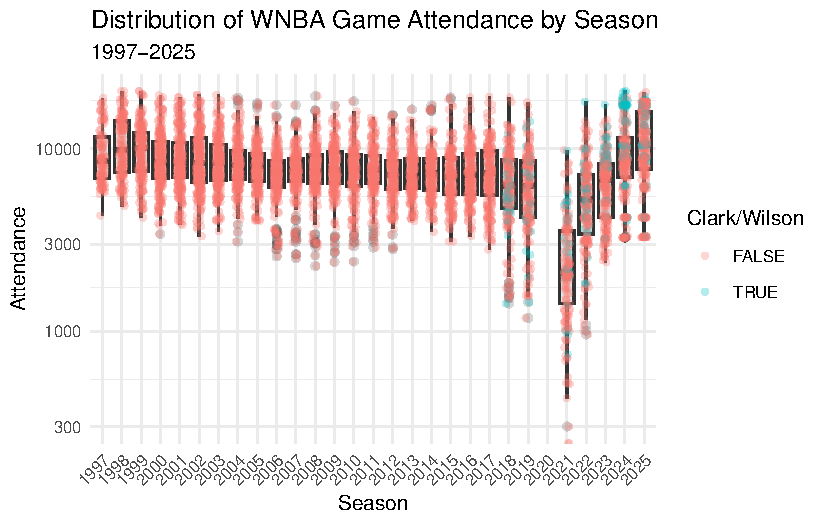
\includegraphics[keepaspectratio]{index_files/figure-pdf/fig-boxplots-1.pdf}}

}

\caption{\label{fig-boxplots}Distribution of WNBA game attendance by
season. Note that the vertical axis has a logarithmic scale. Caitlin
Clark and/or A'ja Wilson's games are separated by color.}

\end{figure}%

\subsection{Arena capacity}\label{arena-capacity}

While we recorded reported arena capacities, those capacities were
difficult to obtain for venues not in current use, they change over
time, and some games had attendance that exceeded the arena's reported
capacity. Thus, we estimate each arena's capacity as the larger of the
reported capacity, or the maximum recorded attendance at that arena in
the sample. This ensures that our figures for the percentage of
estimated arena capacity are bounded above by 1.

We designate a sellout as a game in which the attendance exceeds 92\% of
the arena's estimated capacity. Using our definition, we deem 3.5\% of
the games to be sellouts, with nearly half of those occurring in the
past two seasons. 38 of Clark's 53 games have sold out.

Figure~\ref{fig-boxplots-capacity} shows the distribution of attendance
as a percentage of the arena's estimated capacity.

\protect\phantomsection\label{cell-fig-boxplots-capacity}
\begin{figure}[H]

\centering{

\pandocbounded{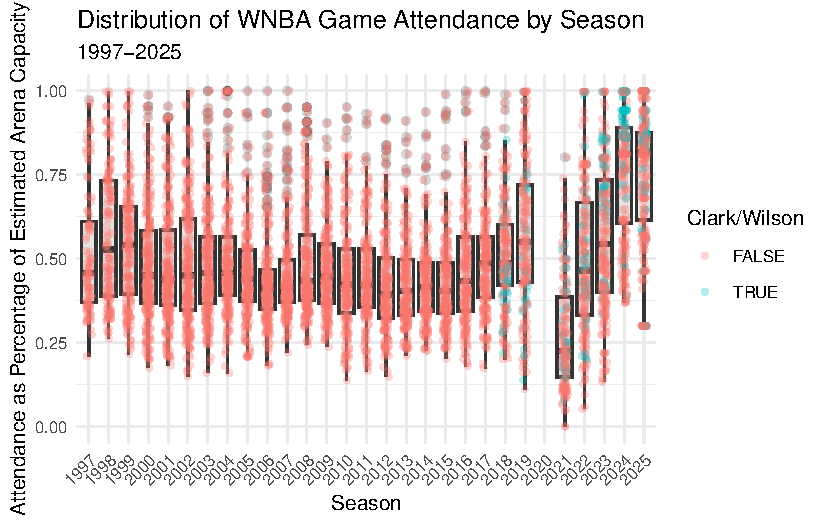
\includegraphics[keepaspectratio]{index_files/figure-pdf/fig-boxplots-capacity-1.pdf}}

}

\caption{\label{fig-boxplots-capacity}Distribution of WNBA game
attendance as a percentage of estimated arena capacity by season. Clark
and Wilson games are highlighted by color.}

\end{figure}%

\subsection{Estimating team strength}\label{sec-elo}

We used the game-level results data to model the evolution of the
strength of each WNBA team over time. Measuring team strength is
necessary to test our hypothesis that attendance is in part driven by
the desire of fans to see quality basketball. We considered
season-to-date winning percentage and a rolling 44-game (the length of a
typical WNBA season) winning percentage before settling on Elo rating
(Elo 1978), because Elo rating updates with each game, and thus more
accurately reflects the information that fans have access to in deciding
to attend games. Originally developed for rating chess players, Elo
rating is well-understood in sports analytics as a measure of team
strength that updates after each game, and---unlike winning percentage
and rolling winning percentage---takes into account not only the outcome
but also the previous estimated team strength of both teams. This means
that beating a team with a higher Elo rating has a greater positive
effect than beating a team with a lower Elo rating, imbuing outcomes
with more nuance than simple win-loss record.

Let \(\theta_{i}(t)\) be the strength of team \(i\) at time \(t\), where
Elo ratings are centered at 1500. Then if the probability that team
\(i\) beats team \(j\) is modeled by a logistic curve with base 10 and
scale factor 400, the win probability is given by: \[
p_{ij}(t) = \Pr(i \text{ beats }j \text{ at time }t) = \frac{1}{1 + 10^{\frac{\theta_{j}(t) -  \theta_{i}(t)  }{400}}} \,.
\]

Each team \(i\) starts the 1997 season with
\(\hat{\theta}_{i}(0) = 1500\), and following each game, team \(i\)'s
rating is updated via the formula \[
  \hat{\theta}_{i}(t+1) = \hat{\theta}_{i}(t) + K \cdot \left[ I(i \text{ beats } j)  - \hat{p}_{ij}(t) \right] 
\] where \(I(i \text{ beats } j)\) is an indicator variable that is 1 if
\(i\) beats \(j\) and \(-1\) if \(j\) beats \(i\), and \(K = 32\) is a
constant that controls how sensitive the ratings are to each game. For
example, suppose team \(i\) has an Elo rating of 1600 and team \(j\)
1450. Then team \(i\) has a 0.703 probability of beating team \(j\) and
if they win, their rating will improve by
\(32 \cdot (1 - \text{0.703}) = \text{9.49}\) points, while team \(j\)'s
rating will decrease by the same amount. Note that if team \(j\) upsets
team \(i\), the corresponding changes in rating will be 22.51 points.
This larger amount reflects the less likely outcome.

We fit Elo ratings using the \textbf{elo} package for R.
Figure~\ref{fig-elo} shows the evolution of Elo rating
\(\hat{\theta}_i(t)\) by franchise for the 12 teams who were active
during the 2024 season. The recent poor performance of the Los Angeles
Sparks, the 2010 dominance of the Seattle Storm, and the recent rise of
the New York Liberty and Indiana Fever are easily visible.

\protect\phantomsection\label{cell-fig-elo}
\begin{figure}[H]

\centering{

\pandocbounded{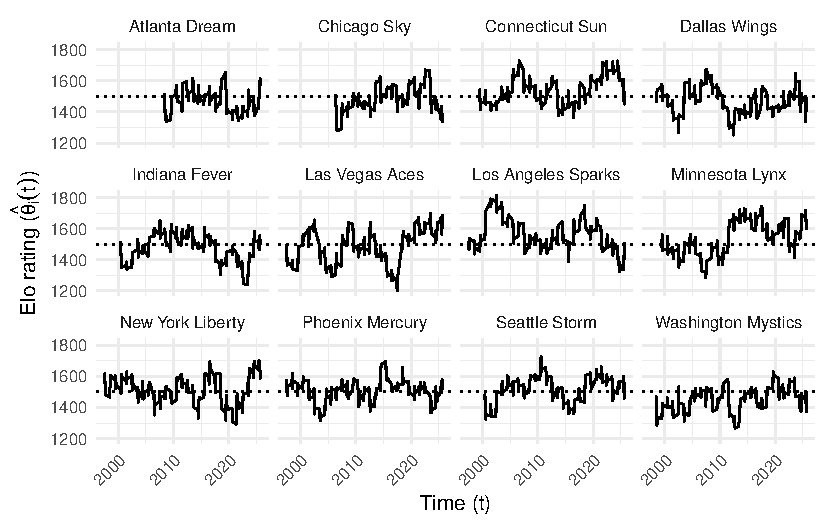
\includegraphics[keepaspectratio]{index_files/figure-pdf/fig-elo-1.pdf}}

}

\caption{\label{fig-elo}Evolution of team Elo ratings in the WNBA
(1997-2025). Only franchises active in 2024 are shown. The recent poor
performance of the Los Angeles Sparks, the 2010 dominance of the Seattle
Storm, and the recent rise of the New York Liberty and Indiana Fever are
easily visible. Note that all franchises begin with a 1500 rating.}

\end{figure}%

\subsection{Estimating home win
probability}\label{estimating-home-win-probability}

We also added a home court advantage equivalent to 60 points (of Elo
rating) to our home win probability model, so that: \[
  \hat{p}_{ij}(t) = \Pr(i \text{ beats }j \text{ at time }t \text{ at home}) = \frac{1}{1 + 10^{\frac{\hat{\theta}_{j}(t) - \left( \hat{\theta}_{i}(t) + 60 \right)  }{400}}} \,.
\] We arrived at 60 points by iteratively calibrating the win
probabilities to match the observed frequencies by minimizing the Brier
score. The model fit very well for most of the games (see
Table~\ref{tbl-calibrate}).

\begin{table}

\caption{\label{tbl-calibrate}Calibration of home win probability model,
based on Elo ratings. We note that in the most frequent situations,
where the home team was a slight favorite, the observed home win
probability is within 3 percentage points of the predicted home
probability. However, in those rarer occasions where a home win was
extremely likely or unlikely, the model was slightly less accurate.}

\centering{

\caption*{
{\fontsize{20}{25}\selectfont  WNBA Home Win Probability Model Calibration (1997-2025)\fontsize{8}{10}\selectfont } \\ 
{\fontsize{14}{17}\selectfont  10 Equally-spaced Bins\fontsize{8}{10}\selectfont }
} 
\fontsize{8.0pt}{10.0pt}\selectfont
\begin{tabular*}{1\linewidth}{@{\extracolsep{\fill}}crrrr}
\toprule
Wpct Bin & Games & Bin Midpoint & Obs Home Wpct & Diff \\ 
\midrule\addlinespace[2.5pt]
(0.102,0.189] & 61 & 0.161 & 0.213 & 0.052 \\ 
(0.189,0.275] & 251 & 0.243 & 0.271 & 0.028 \\ 
(0.275,0.361] & 422 & 0.322 & 0.384 & 0.062 \\ 
(0.361,0.446] & 691 & 0.405 & 0.454 & 0.050 \\ 
(0.446,0.532] & 970 & 0.492 & 0.520 & 0.029 \\ 
(0.532,0.618] & 1,104 & 0.577 & 0.601 & 0.024 \\ 
(0.618,0.704] & 1,080 & 0.660 & 0.661 & 0.001 \\ 
(0.704,0.789] & 925 & 0.742 & 0.706 & -0.036 \\ 
(0.789,0.875] & 525 & 0.825 & 0.775 & -0.050 \\ 
(0.875,0.962] & 135 & 0.896 & 0.889 & -0.007 \\ 
\bottomrule
\end{tabular*}

}

\end{table}%

\section{Methods}\label{methods}

\subsection{Response variables}\label{response-variables}

Our goal is to model the attendance (\(y\)) at a given WNBA game, as a
function of several different measures of fan engagement detailed in
Section~\ref{sec-fan}. We also include several control variables to
account for time and city-related effects (see
Section~\ref{sec-control}).

Since we know the arena in which the game took place and the capacity of
that arena, we also developed an alternative response variable:
percentage of estimated arena capacity filled (\(\gamma\)).

In Figure~\ref{fig-attendance-year}, we observe the relationship between
attendance and estimated home win probability. We add a simple quadratic
regression line to reflect the quadratic relationship posited by Coates
et al. (2014). In most years, the slope appears to be positive and the
curvature concave up.

\begin{tcolorbox}[enhanced jigsaw, arc=.35mm, bottomrule=.15mm, bottomtitle=1mm, breakable, colback=white, colbacktitle=quarto-callout-note-color!10!white, colframe=quarto-callout-note-color-frame, coltitle=black, left=2mm, leftrule=.75mm, opacityback=0, opacitybacktitle=0.6, rightrule=.15mm, title=\textcolor{quarto-callout-note-color}{\faInfo}\hspace{0.5em}{Ben}, titlerule=0mm, toprule=.15mm, toptitle=1mm]

How does this compare to Coates, et al?

\end{tcolorbox}

\protect\phantomsection\label{cell-fig-attendance-year}
\begin{figure}[H]

\centering{

\pandocbounded{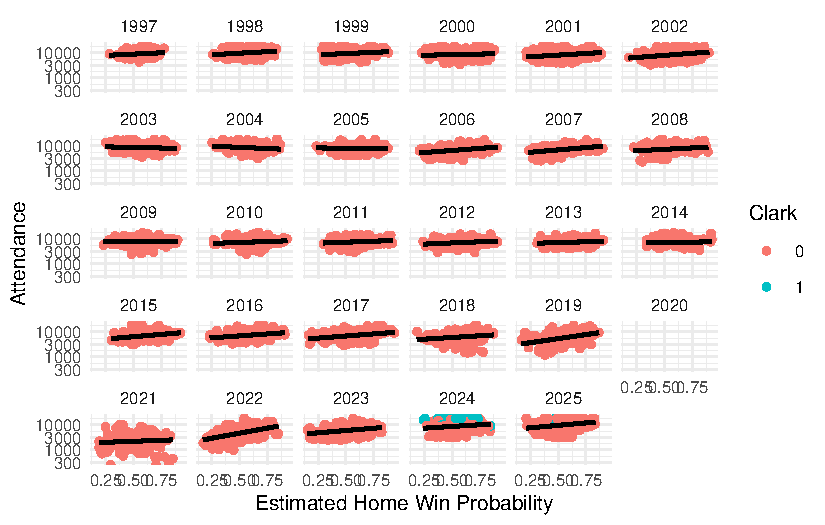
\includegraphics[keepaspectratio]{index_files/figure-pdf/fig-attendance-year-1.pdf}}

}

\caption{\label{fig-attendance-year}WNBA attendance by season against
estimated home win probability. We note that in most years, the slope of
the association appears to be positive and the curvature concave up.}

\end{figure}%

In Figure~\ref{fig-capacity-year}, we note similar trends in the
relationship between the percentage of the estimated arena capacity
filled and the estimated home win probability. We also note that since
the percentage of arena capacity cannot exceed 1, there are edge effects
created by sellouts. Those sellouts are much more frequent in the last
two years of data, and many of the sellouts involve Caitlin Clark.

\protect\phantomsection\label{cell-fig-capacity-year}
\begin{figure}[H]

\centering{

\pandocbounded{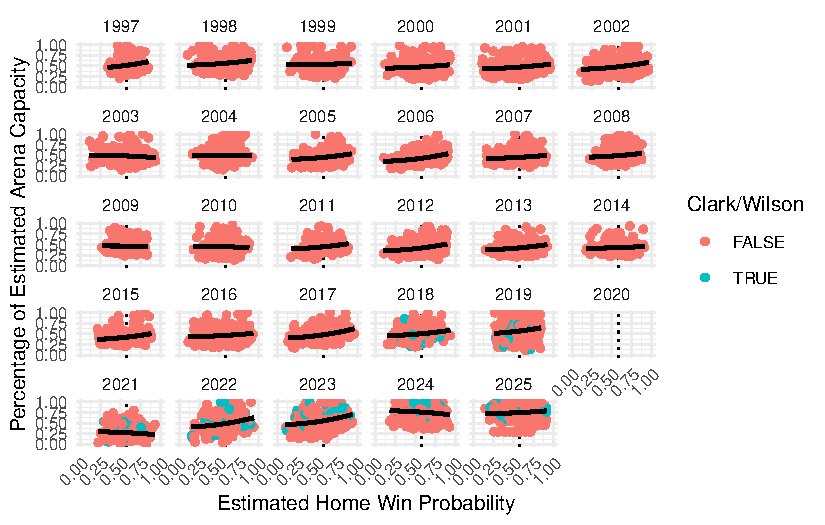
\includegraphics[keepaspectratio]{index_files/figure-pdf/fig-capacity-year-1.pdf}}

}

\caption{\label{fig-capacity-year}WNBA percentage of estimated arena
capacity filled by season, against estimated home win probability. We
note the edge effects caused by sellouts, which occur much more
frequently in 2024 and 2025.}

\end{figure}%

Table~\ref{tbl-sellout} summarizes attendance figures across the 10
arenas with the most sellouts. We make several observations. The Golden
State Valkyries (a 2025 expansion franchise) sold out all 22 of their
games at the Chase Center. In terms of measuring fan demand, there is a
profound difference between selling out a small arena (e.g., the
Entertainment and Sports Arena in Washington, D.C. with a capacity of
slightly more than 4000) and a large arena (e.g., Gainbridge Fieldhouse
in Indianapolis, with a capacity of more than 18000). Teams like
Washington and Connecticut, in order to generate more excitement in the
arena and positive images on telecasts, may have been trying to maximize
the percentage of arena capacity at the expense of drawing larger
crowds. Or perhaps they didn't have a larger arena in which to play.
Just two of the 27 sellouts at Gainbridge Fieldhouse occurred before
Clark's arrival.

{

\begin{longtable}[]{@{}
  >{\raggedright\arraybackslash}p{(\linewidth - 14\tabcolsep) * \real{0.2562}}
  >{\raggedright\arraybackslash}p{(\linewidth - 14\tabcolsep) * \real{0.0909}}
  >{\raggedleft\arraybackslash}p{(\linewidth - 14\tabcolsep) * \real{0.0826}}
  >{\raggedleft\arraybackslash}p{(\linewidth - 14\tabcolsep) * \real{0.1240}}
  >{\raggedleft\arraybackslash}p{(\linewidth - 14\tabcolsep) * \real{0.1240}}
  >{\raggedleft\arraybackslash}p{(\linewidth - 14\tabcolsep) * \real{0.1074}}
  >{\raggedleft\arraybackslash}p{(\linewidth - 14\tabcolsep) * \real{0.1074}}
  >{\raggedleft\arraybackslash}p{(\linewidth - 14\tabcolsep) * \real{0.1074}}@{}}

\caption{\label{tbl-sellout}Summary statistics for attendance across the
10 WNBA arenas with the most sellouts. We note the difference between
selling out a small arena (e.g., Entertainment and Sports Arena in
Washington, D.C.) and a large arena (e.g., Gainbridge Fieldhouse in
Indianapolis).}

\tabularnewline

\toprule\noalign{}
\begin{minipage}[b]{\linewidth}\raggedright
Arena
\end{minipage} & \begin{minipage}[b]{\linewidth}\raggedright
Home Teams
\end{minipage} & \begin{minipage}[b]{\linewidth}\raggedleft
Num Games
\end{minipage} & \begin{minipage}[b]{\linewidth}\raggedleft
Max Attendance
\end{minipage} & \begin{minipage}[b]{\linewidth}\raggedleft
Avg Attendance
\end{minipage} & \begin{minipage}[b]{\linewidth}\raggedleft
Num Sellouts
\end{minipage} & \begin{minipage}[b]{\linewidth}\raggedleft
Pct Sellouts
\end{minipage} & \begin{minipage}[b]{\linewidth}\raggedleft
Avg Capacity
\end{minipage} \\
\midrule\noalign{}
\endhead
\bottomrule\noalign{}
\endlastfoot
Entertainment and Sports Arena & WAS & 84 & 4210 & 3578.3 & 47 & 0.56 &
0.85 \\
Gainbridge Fieldhouse & IND & 404 & 18345 & 8573.0 & 27 & 0.07 & 0.47 \\
Chase Center & GSV & 22 & 18064 & 18064.0 & 22 & 1.00 & 1.00 \\
Mohegan Sun Arena & CON & 381 & 9518 & 6690.8 & 16 & 0.04 & 0.70 \\
Barclays Center & NYL & 97 & 17758 & 9288.1 & 14 & 0.14 & 0.52 \\
Capital One Arena & WAS & 357 & 20711 & 10673.8 & 14 & 0.04 & 0.52 \\
Crypto.com Arena & LAS & 401 & 19282 & 9645.7 & 10 & 0.02 & 0.50 \\
Compaq Center & HOU & 144 & 16285 & 10265.2 & 9 & 0.06 & 0.63 \\
ARCO Arena & SAC & 212 & 17317 & 8324.1 & 7 & 0.03 & 0.48 \\
Madison Square Garden & NYL & 292 & 19563 & 11347.6 & 6 & 0.02 & 0.58 \\
Total among 60 arenas & 19 & 6164 & 20711 & 8076.6 & 218 & 0.04 &
0.39 \\

\end{longtable}

}

\subsection{Modeling fan engagement}\label{sec-fan}

In Section~\ref{sec-elo}, we described our use of Elo rating to estimate
the strength of the home team (\(\hat{\theta}_i(t)\)), the strength of
the visiting team (\(\hat{\theta}_j(t)\)) and the home win probability
(\(\hat{p}_{ij}(t)\)) (which is itself a function of the estimated team
strengths).

As noted in Section~\ref{sec-intro}, there are multiple notions of what
drives fan engagement relevant to the WNBA. Each of these notions can be
captured by a simple bivariate function of the corresponding strengths
of the teams
\(f_k(i, j, t) = f_k(\hat{\theta}_i(t), \hat{\theta}_j(t))\). The first
and third have been rescaled so that they will have means close to 0.

\begin{itemize}
\tightlist
\item
  Quality of play: fans may wish to attend a game in person if they
  expect the quality of play to be high. We model this as the product of
  the Elo rating of the two teams
  (\(f_1(i, j, t) = \hat{\theta}_i(t) \cdot \hat{\theta}_j(t)\))
\item
  Uncertainty of outcome: fans may wish to attend a game for which the
  outcome is uncertain. We model this as negative square root of the
  absolute difference in the two teams' Elo ratings:
  (\(f_2(i, j, t) = -\sqrt{|\hat{\theta}_i(t) - \hat{\theta}_j(t)|}\)).
  The negative sign ensures that closely-matched opponents will have the
  highest values, and the square root helps to make the spread more
  symmetric.\footnote{It is possible that this formulation might
    misidentify how fans view outcome uncertainty. That is, fans might
    not seek exactly equal team strength across the two opponents, but
    rather would be just as satisfied as long as there is sufficient
    uncertainty.}
\item
  Loss aversion: fans may wish to attend a game to see their team (the
  home team) win. We model this using the estimated home win probability
  function above (\(f_3(i, j, t) = (\hat{p}_{ij}(t))^2\)). Note that
  this term is nonlinear as in Coates et al. (2014).
\end{itemize}

The distribution of attendance with respect to \(f_1\) and \(f_2\) are
shown in Figure~\ref{fig-attend-f1} and Figure~\ref{fig-attend-f2},
respectively, with the corresponding plots for percentage of estimated
arena capacity shown in Figure~\ref{fig-capacity-f1} and
Figure~\ref{fig-capacity-f2}.

\subsubsection{Normalization}\label{normalization}

Figure~\ref{fig-rescaled} shows the distribution of our fan engagement
variables after normalizing
(\(Z_k = \frac{f_k - \mu(f_k)}{\sigma(f_k)}\)). We note that
Table~\ref{tbl-cor} shows that our three fan engagement variables are
largely uncorrelated.

{

\begin{longtable}[]{@{}
  >{\raggedright\arraybackslash}p{(\linewidth - 6\tabcolsep) * \real{0.2692}}
  >{\raggedleft\arraybackslash}p{(\linewidth - 6\tabcolsep) * \real{0.2436}}
  >{\raggedleft\arraybackslash}p{(\linewidth - 6\tabcolsep) * \real{0.2692}}
  >{\raggedleft\arraybackslash}p{(\linewidth - 6\tabcolsep) * \real{0.2179}}@{}}

\caption{\label{tbl-cor}Correlations among normalized fan engagment
variables.}

\tabularnewline

\toprule\noalign{}
\begin{minipage}[b]{\linewidth}\raggedright
\end{minipage} & \begin{minipage}[b]{\linewidth}\raggedleft
Z1 Quality of Play
\end{minipage} & \begin{minipage}[b]{\linewidth}\raggedleft
Z2 Uncertain Outcome
\end{minipage} & \begin{minipage}[b]{\linewidth}\raggedleft
Z3 Loss Aversion
\end{minipage} \\
\midrule\noalign{}
\endhead
\bottomrule\noalign{}
\endlastfoot
Z1 Quality of Play & 1.000 & -0.022 & -0.003 \\
Z2 Uncertain Outcome & -0.022 & 1.000 & -0.103 \\
Z3 Loss Aversion & -0.003 & -0.103 & 1.000 \\

\end{longtable}

}

Figure~\ref{fig-all-z} illustrates how our normalized measures of fan
engagement vary with respect to the estimated (pregame) strength of the
home and away teams. The lack of correlation across these measures
reported in Table~\ref{tbl-cor} is apparent graphically. The 4th panel
in Figure~\ref{fig-all-z} shows the simple sum of the three measures of
fan engagement. Although this metric is not used directly in our
analysis, it might be considered a composite of three competing,
uncorrelated notions of fan engagement.

\protect\phantomsection\label{cell-fig-all-z}
\begin{figure}[H]

\centering{

\pandocbounded{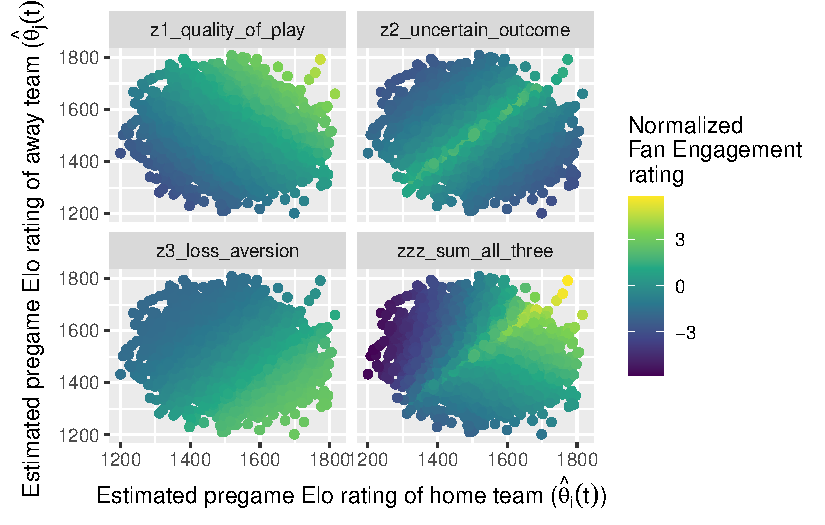
\includegraphics[keepaspectratio]{index_files/figure-pdf/fig-all-z-1.pdf}}

}

\caption{\label{fig-all-z}Distribution of normalized fan engagment
measures as a function of home and away pregrame Elo ratings. The lack
of correlation across these measures is obvious. The 4th panel shows the
simple sum of all three measures.}

\end{figure}%

\subsection{Control variables}\label{sec-control}

As time-related control variables, we include the season (\(\tau_1\)),
the month of the year (\(\tau_2\)), and day of the week (\(\tau_3\)) as
fixed effects. To control for city-related effects, we also include the
team name (\(\phi_1\)), as well as the metropolitan area median income
(\(\phi_2\), in thousands of USD) and population (\(\phi_3\), in
millions) of the home city\footnote{The data for the population and the
  median income of cities comes from the American Community Survey,
  access to which was provided in R by the \textbf{tidycensus} package.
  Because the population and median income statistics were available at
  irregular time periods (due to the COVID-19 pandemic and other
  factors), impute missing values using a cubic spline for interpolated
  values and the last observation carried forward (or backward) for
  extraploted values.}. Finally, we include an indicator based on
whether Caitlin Clark or A'ja Wilson played more than 0 minutes in the
game (\(\chi_1, \chi_2\), respectively).

\subsection{Interaction}\label{interaction}

Testing our primary hypotheses requires analyzing how the relationships
between attendance and fan engagement have changed over time. To capture
these changes, we include interaction terms between our measures of fan
engagement (\(f_k\)) and season (\(\tau_1\)).

\subsection{Model formulation for attendance}\label{sec-mod-attend}

Because the raw attendance figures are not normally distributed, we
model the logarithm of attendance. Similarly, because the percentage of
arena capacity are bound above by 1 and below by 0, we employ a Tobit
regression model.

Like Coates et al. (2014), we model the natural logarithm of attendance.

Our general regression model for attendance is: \begin{align*}
  \ln{y} &= \beta_0 + \underbrace{\beta_2 Z_1 + \beta_3 Z_2 + \beta_4 Z_3}_{\text{fan engagement}} \\
    &+ \underbrace{\beta_5 \tau_1 + \beta_6 \tau_2 + \beta_7 \tau_3}_{\text{time-related}} + \underbrace{\beta_8 \phi_1 + \beta_9 \phi_2 + \beta_{10} \phi_3}_{\text{ city-related }} \\
    &+ \underbrace{\beta_{11} \chi_1 + \beta_{12} \chi_2}_{\text{player-related}} + \underbrace{\beta_{13} Z_1 \tau_1 + \beta_{14} Z_2 \tau_2 + \beta_{15} Z_3 \tau_3}_{\text{interaction}} + \epsilon \\
    &= \symbf{X} \symbf{\beta} + \epsilon \,,
\end{align*} where \(\beta_j \in \mathbb{R}\) for
\(j = \{0, 1, 2, 3, 11, 12\}\), while the other \(\beta_j\) coefficients
are vectors of length equal to the number of factor levels in their
corresponding categorical explanatory variable minus 1. Most notably
\(\beta_5\) and \(\beta_8\) have 26 values (corresponding to each season
after 1997) and \(\beta_5\) has 12 values (corresponding to each team).
Only current WNBA franchises are included in the regression model. We
also excluded all data from the 2020 and 2021 seasons, since there were
no fans allowed in all or parts of both seasons.

\begin{tcolorbox}[enhanced jigsaw, arc=.35mm, bottomrule=.15mm, bottomtitle=1mm, breakable, colback=white, colbacktitle=quarto-callout-note-color!10!white, colframe=quarto-callout-note-color-frame, coltitle=black, left=2mm, leftrule=.75mm, opacityback=0, opacitybacktitle=0.6, rightrule=.15mm, title=\textcolor{quarto-callout-note-color}{\faInfo}\hspace{0.5em}{Ben}, titlerule=0mm, toprule=.15mm, toptitle=1mm]

Need to add details about Tobit modeling.

\end{tcolorbox}

We fit the Tobit model in R using the \texttt{vglm()} and
\texttt{tobit()} functions from the \textbf{VGAM} package.

\subsection{Model formulation for percentage of arena
capacity}\label{sec-mod-cap}

We fit the same model with \(\gamma\) as the response, but because our
response variable \(\gamma\) is constrained between 0 and 1 and has
significant mass at 1 exactly, we use the Papke-Wooldridge fractional
response model (Papke and Wooldridge 1996). This is equivalent to
fitting a generalized linear model with a logit link function and
applying HC1 sandwich estimators (MacKinnon and White 1985) for the
covariance matrix, which we accomplish using the \textbf{sandwich}
package in R. \[
  \mathbb{E}{(\gamma | \symbf{X})} = G(\symbf{X} \symbf{\eta}) \,,
\] where \(G(z) = \frac{e^z}{1 + e^z}\) is the (vectorized) logistic
function, \(\symbf{X}\) is as above, and \(\symbf{\eta}\) has the same
structure as \(\symbf{\beta}\) defined above.

\section{Results}\label{results}

In keeping with recent guidance from Wasserstein and Lazar (2016) and
Wasserstein et al. (2019), and with a sample size of over 5000
observations and dozens of coefficients, we are less interested in the
p-values shown in Table~\ref{tbl-coefs}, and focus our attention on the
magnitude and practical impact of the fitted coefficients. (All
variables except for population achieve ``statistical significance'' at
the 5\%-level, as shown in Table~\ref{tbl-anova-tobit}).

\subsection{Modeling attendance}\label{sec-attend}

\subsubsection{Baseline effects}\label{baseline-effects}

Table~\ref{tbl-coefs} reports estimates from the Tobit model. Because
each measure of fan engagement interacts with season, the reported
coefficients for quality of play, outcome uncertainty, and loss aversion
represent their estimated effects for the reference levels: a home game
for the Atlanta Dream taking place on a Sunday in May (in which neither
Clark nor Wilson is playing). The interaction terms, discussed in
Section~\ref{sec-annual}, capture how these relationships evolve over
time.

{

\begin{longtable}[]{@{}
  >{\raggedright\arraybackslash}p{(\linewidth - 12\tabcolsep) * \real{0.3000}}
  >{\raggedleft\arraybackslash}p{(\linewidth - 12\tabcolsep) * \real{0.1125}}
  >{\raggedleft\arraybackslash}p{(\linewidth - 12\tabcolsep) * \real{0.1250}}
  >{\raggedleft\arraybackslash}p{(\linewidth - 12\tabcolsep) * \real{0.1250}}
  >{\raggedleft\arraybackslash}p{(\linewidth - 12\tabcolsep) * \real{0.1000}}
  >{\raggedleft\arraybackslash}p{(\linewidth - 12\tabcolsep) * \real{0.1125}}
  >{\raggedleft\arraybackslash}p{(\linewidth - 12\tabcolsep) * \real{0.1250}}@{}}

\caption{\label{tbl-coefs}Fitted coefficients for scalar terms in Tobit
model for the natural logarithm of attendance.}

\tabularnewline

\toprule\noalign{}
\begin{minipage}[b]{\linewidth}\raggedright
Term
\end{minipage} & \begin{minipage}[b]{\linewidth}\raggedleft
Estimate
\end{minipage} & \begin{minipage}[b]{\linewidth}\raggedleft
Std Error
\end{minipage} & \begin{minipage}[b]{\linewidth}\raggedleft
Statistic
\end{minipage} & \begin{minipage}[b]{\linewidth}\raggedleft
P Value
\end{minipage} & \begin{minipage}[b]{\linewidth}\raggedleft
Conf Low
\end{minipage} & \begin{minipage}[b]{\linewidth}\raggedleft
Conf High
\end{minipage} \\
\midrule\noalign{}
\endhead
\bottomrule\noalign{}
\endlastfoot
(Intercept):1 & 9.185 & 0.085 & 107.839 & 0.000 & 9.018 & 9.352 \\
(Intercept):2 & -1.181 & 0.010 & -117.733 & 0.000 & -1.201 & -1.162 \\
I(z1\_quality\_of\_play) & 0.212 & 0.079 & 2.677 & 0.007 & 0.057 &
0.368 \\
I(z2\_uncertain\_outcome) & 0.019 & 0.045 & 0.430 & 0.667 & -0.069 &
0.108 \\
I(z3\_loss\_aversion) & 0.025 & 0.056 & 0.440 & 0.660 & -0.085 &
0.135 \\
Player: A'ja Wilson & 0.048 & 0.026 & 1.828 & 0.068 & -0.003 & 0.099 \\
Player: Caitlin Clark & 0.846 & 0.054 & 15.543 & 0.000 & 0.739 &
0.953 \\
median\_income & -0.006 & 0.001 & -4.169 & 0.000 & -0.008 & -0.003 \\
metro\_pop & -0.016 & 0.006 & -2.586 & 0.010 & -0.029 & -0.004 \\

\end{longtable}

}

In the reference season, the evidence for loss aversion (\(Z_3\)) and
uncertainty of outcome (\(Z_2\)) is weak, with those coefficients being
of little significance, either practically or statistically. The
coefficient for quality of play (which \emph{is} statistically
significant) suggest that in 1997, a 1 standard deviation increase in
the quality of play (as measured by the product of the Elo ratings) is
associated with a modest 2.15\% increase in the expected attendance,
after controlling for our other factors. The strong support for quality
of play (relative to uncertainty of outcome and loss aversion) is a key
finding.

Games featuring Caitlin Clark were associated with significantly higher
attendance, while A'ja Wilson's presence was associated with a smaller
but still nontrivial increase in attendance. The expected attendance
more than doubles (i.e., is multiplied by \(\exp(\text{0.846})\) = 2.33)
when Clark plays in the game, and this is \emph{after} controlling for
the Indiana Fever team effect, the level of fan engagement, and the
season effects! The corresponding change in attendance for A'ja
Wilson---by most accounts a better player than Clark---is multiplying by
just 1.05.

\begin{tcolorbox}[enhanced jigsaw, arc=.35mm, bottomrule=.15mm, bottomtitle=1mm, breakable, colback=white, colbacktitle=quarto-callout-note-color!10!white, colframe=quarto-callout-note-color-frame, coltitle=black, left=2mm, leftrule=.75mm, opacityback=0, opacitybacktitle=0.6, rightrule=.15mm, title=\textcolor{quarto-callout-note-color}{\faInfo}\hspace{0.5em}{Ben}, titlerule=0mm, toprule=.15mm, toptitle=1mm]

Need to provide an interpretation for the Tobit coefficient.

\end{tcolorbox}

Among the control variables, median income and metro area population had
small negative effects after controlling for other variables.

Figure~\ref{fig-attend-coefs} presents the results of
Table~\ref{tbl-coefs} and some additional coefficients graphically.
Confidence intervals for the coefficient associated with the Golden
State Valkyries is omitted because it was so large that it renders all
of the other effects indistinguishable. The New York Liberty have the
largest team effect, and all teams are positive relative to the Dream.
Saturday games have the highest attendance, as do games later in the
season.

\protect\phantomsection\label{cell-fig-attend-coefs}
\begin{figure}[H]

\centering{

\pandocbounded{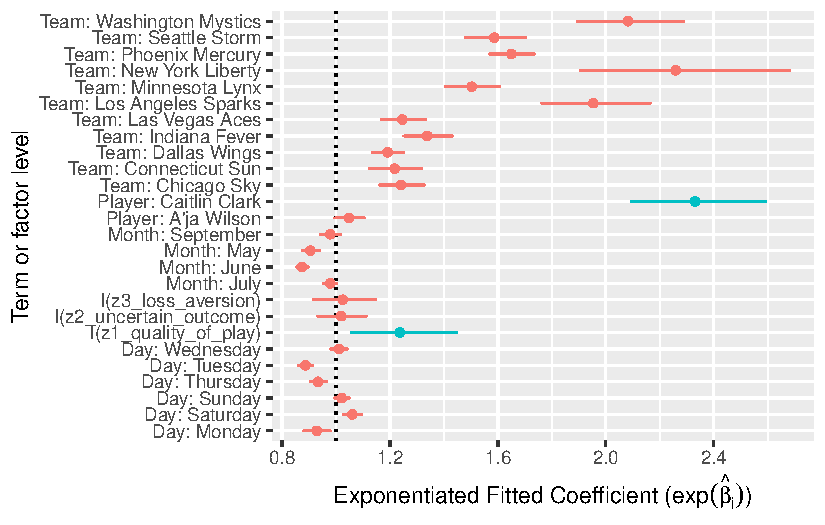
\includegraphics[keepaspectratio]{index_files/figure-pdf/fig-attend-coefs-1.pdf}}

}

\caption{\label{fig-attend-coefs}Relative magnitudes of fitted
coefficients in attendance model, with 95\% confidence intervals. The
coefficient for the Golden State Valkyries is omitted. Coefficients of
interest are highlighted in green. Note the relatively large size of the
coefficient associated with Caitlin Clark.}

\end{figure}%

Table~\ref{tbl-glance} characterizes the model's fit.

\subsubsection{Annual effects}\label{sec-annual}

Table~\ref{tbl-lrt} shows a likelihood ratio test between our model and
a reduced model that does not include the interaction terms. The
interactions introduce 78 additional terms corresponding to season
specific slopes to our model. The likelihood ratio test rejects the null
hypothesis that all season-specific changes in slope are equal to zero,
indicating that the effects of our fan engagement measures differ
significantly across seasons.

The ANOVA tables shown in Table~\ref{tbl-anova-tobit} further support
the inclusion of all three sets of interaction terms.

{

\begin{longtable}[]{@{}rrrrr@{}}

\caption{\label{tbl-lrt}Model comparison: constant vs season-varying
effects of fan engagement on attendance.}

\tabularnewline

\toprule\noalign{}
Resid. Df & LogLik & Df & 2 * LogLik Diff. & Pr(\textgreater Chi) \\
\midrule\noalign{}
\endhead
\bottomrule\noalign{}
\endlastfoot
10069 & -1481.836 & NA & NA & NA \\
9991 & -1283.677 & 78 & 396.318 & 0 \\

\end{longtable}

}

Figure~\ref{fig-season-coefs} isolates the change in intercept
associated with each WNBA season. These reveal that even after
controlling for our others variables---including the Caitlin Clark
effect---expected attendance has exceeded its 1997 baseline in the most
recent seasons. Thus, after controlling for the influence of Clark and
Wilson, league expected attendance has fully recovered from the COVID-19
pandemic and the malaise of the early 2000s and 2010s.

\protect\phantomsection\label{cell-fig-season-coefs}
\begin{figure}[H]

\centering{

\pandocbounded{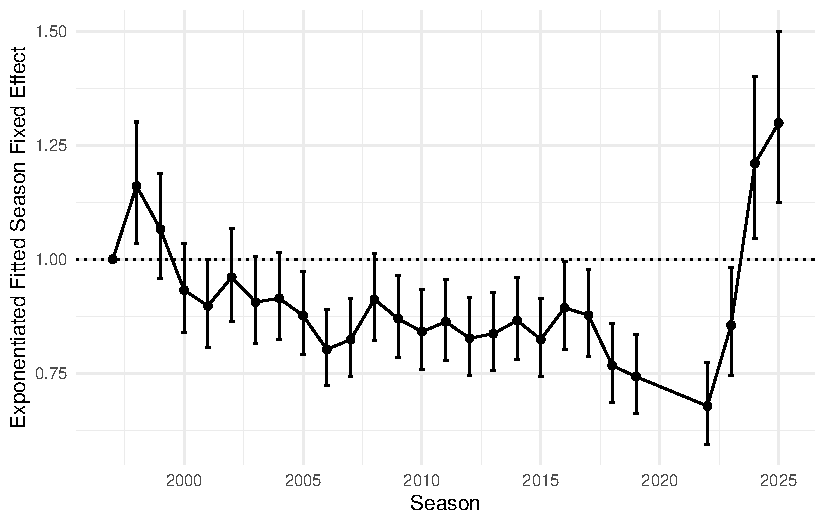
\includegraphics[keepaspectratio]{index_files/figure-pdf/fig-season-coefs-1.pdf}}

}

\caption{\label{fig-season-coefs}Estimated season-level fixed effects
for Tobit attendance model.}

\end{figure}%

Figure~\ref{fig-season-slopes} shows the exponentiated season-by-season
combined slopes for our three measures of fan engagement. The initial
values (corresponding to 1997), match those in Table~\ref{tbl-coefs},
and the subsequent interaction terms modify the relationships between
attendance and fan engagement. In Figure~\ref{fig-season-slopes}, we can
see that there is little to no association with attendance from the
uncertainty of the outcome.\footnote{See the previous note about
  possible misspecification of the uncertainty of outcome response.} The
slope associated with loss aversion always positive and generally
increasing, suggesting that the attendance response to home win
probability has strengthened over the league's history. This suggests
that fan behavior in the WNBA may be becoming more similar to the
behavior observed in MLB by Coates et al. (2014).

\begin{tcolorbox}[enhanced jigsaw, arc=.35mm, bottomrule=.15mm, bottomtitle=1mm, breakable, colback=white, colbacktitle=quarto-callout-note-color!10!white, colframe=quarto-callout-note-color-frame, coltitle=black, left=2mm, leftrule=.75mm, opacityback=0, opacitybacktitle=0.6, rightrule=.15mm, title=\textcolor{quarto-callout-note-color}{\faInfo}\hspace{0.5em}{Ben}, titlerule=0mm, toprule=.15mm, toptitle=1mm]

Say something about how this tracks with Agha and Berri.

\end{tcolorbox}

Similarly, the slope associated with quality of play is always positive
and generally increasing, following a steep fall after the league's
first season.

\begin{tcolorbox}[enhanced jigsaw, arc=.35mm, bottomrule=.15mm, bottomtitle=1mm, breakable, colback=white, colbacktitle=quarto-callout-note-color!10!white, colframe=quarto-callout-note-color-frame, coltitle=black, left=2mm, leftrule=.75mm, opacityback=0, opacitybacktitle=0.6, rightrule=.15mm, title=\textcolor{quarto-callout-note-color}{\faInfo}\hspace{0.5em}{Ben}, titlerule=0mm, toprule=.15mm, toptitle=1mm]

I'm not sure why the quality of play initial coefficient is so high and
then drops off.

\end{tcolorbox}

In the case of quality of play and loss aversion, the exponentiated
fitted coefficient value of approximately 0.1 in recent years means that
a one standard deviation increase in these measures is associated with
an increase in attendance that is about 10\% higher than it would have
been in the league's early years. This is another key finding.

\protect\phantomsection\label{cell-fig-season-slopes}
\begin{figure}[H]

\centering{

\pandocbounded{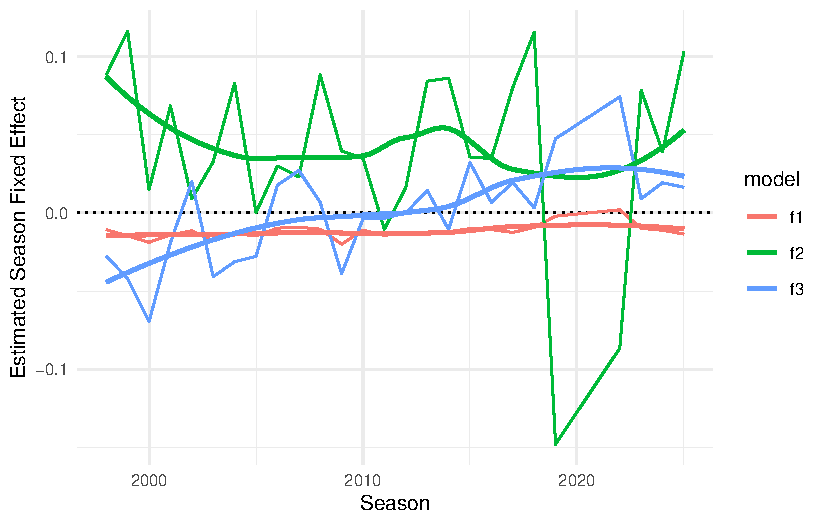
\includegraphics[keepaspectratio]{index_files/figure-pdf/fig-season-slopes-1.pdf}}

}

\caption{\label{fig-season-slopes}Exponentiated fitted combined (main
effect + interaction effect) slope coefficients for Tobit model, by
season.}

\end{figure}%

\subsection{Modeling percentage of arena
capacity}\label{modeling-percentage-of-arena-capacity}

Because our response variable \(\gamma\) is constrained between 0 and 1,
but has significant mass at 1 exactly, we fit a Papke-Wooldridge
fractional response model (Papke and Wooldridge 1996) with HC1 sandwich
estimators for the covariance matrix.

\subsubsection{Main effects}\label{main-effects}

Table~\ref{tbl-coefs2} reports the coefficients from the percentage of
arena capacity models.

{

\begin{longtable}[]{@{}
  >{\raggedright\arraybackslash}p{(\linewidth - 12\tabcolsep) * \real{0.3000}}
  >{\raggedleft\arraybackslash}p{(\linewidth - 12\tabcolsep) * \real{0.1125}}
  >{\raggedleft\arraybackslash}p{(\linewidth - 12\tabcolsep) * \real{0.1250}}
  >{\raggedleft\arraybackslash}p{(\linewidth - 12\tabcolsep) * \real{0.1250}}
  >{\raggedleft\arraybackslash}p{(\linewidth - 12\tabcolsep) * \real{0.1000}}
  >{\raggedleft\arraybackslash}p{(\linewidth - 12\tabcolsep) * \real{0.1125}}
  >{\raggedleft\arraybackslash}p{(\linewidth - 12\tabcolsep) * \real{0.1250}}@{}}

\caption{\label{tbl-coefs2}Table of coefficients from percentage of
arena capacity models.}

\tabularnewline

\toprule\noalign{}
\begin{minipage}[b]{\linewidth}\raggedright
Term
\end{minipage} & \begin{minipage}[b]{\linewidth}\raggedleft
Estimate
\end{minipage} & \begin{minipage}[b]{\linewidth}\raggedleft
Std Error
\end{minipage} & \begin{minipage}[b]{\linewidth}\raggedleft
Statistic
\end{minipage} & \begin{minipage}[b]{\linewidth}\raggedleft
P Value
\end{minipage} & \begin{minipage}[b]{\linewidth}\raggedleft
Conf Low
\end{minipage} & \begin{minipage}[b]{\linewidth}\raggedleft
Conf High
\end{minipage} \\
\midrule\noalign{}
\endhead
\bottomrule\noalign{}
\endlastfoot
(Intercept) & -0.495 & 0.184 & -2.695 & 0.007 & -0.855 & -0.135 \\
I(z1\_quality\_of\_play) & 0.506 & 0.181 & 2.793 & 0.005 & 0.151 &
0.862 \\
I(z2\_uncertain\_outcome) & 0.136 & 0.097 & 1.396 & 0.163 & -0.055 &
0.326 \\
I(z3\_loss\_aversion) & 0.099 & 0.110 & 0.902 & 0.367 & -0.116 &
0.315 \\
Player: A'ja Wilson & 0.275 & 0.064 & 4.329 & 0.000 & 0.151 & 0.400 \\
Player: Caitlin Clark & 1.917 & 0.114 & 16.809 & 0.000 & 1.694 &
2.141 \\
median\_income & 0.006 & 0.003 & 1.844 & 0.065 & 0.000 & 0.012 \\
metro\_pop & 0.111 & 0.012 & 8.954 & 0.000 & 0.086 & 0.135 \\

\end{longtable}

}

Figure~\ref{fig-pct-coefs} shows that\ldots{}

\protect\phantomsection\label{cell-fig-pct-coefs}
\begin{figure}[H]

\centering{

\pandocbounded{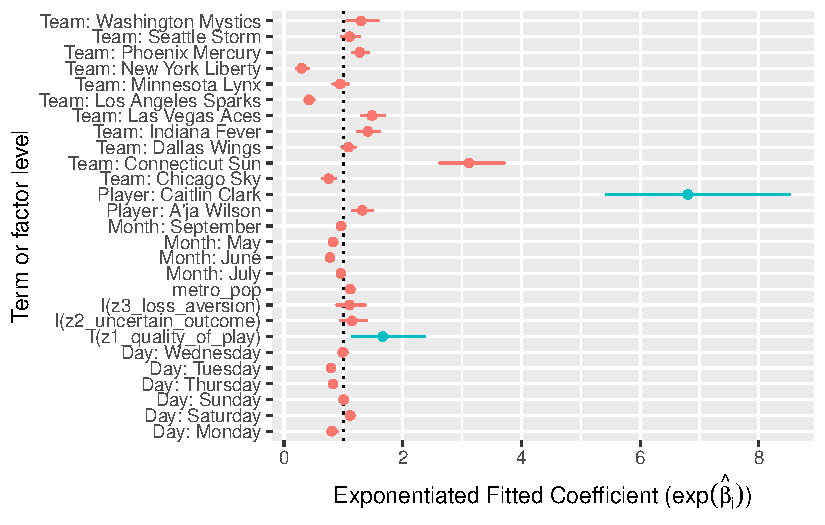
\includegraphics[keepaspectratio]{index_files/figure-pdf/fig-pct-coefs-1.pdf}}

}

\caption{\label{fig-pct-coefs}Relative magnitudes of coefficients in
attendance model. Coefficients of interest are highlighted. Note the
relatively large size of the coefficient associated with Caitlin Clark.}

\end{figure}%

Table~\ref{tbl-glance2} and Table~\ref{tbl-anova2} show model fit
metrics and analysis of variance for the percentage of estimated arena
capacity models, respectively.

\subsubsection{Annual effects}\label{annual-effects}

Figure~\ref{fig-season-coefs2} displays the estimated effects of our fan
engagement measures on attendance relative to the 1997 reference season.
Similar to the overall attendance trends, these effects generally
remained below their 1997 levels for much of the league's history and
only returned to comparable levels recently. In the most recent years of
measurement, however, we see the league exceeding previously
record-holding levels.

\protect\phantomsection\label{cell-fig-season-coefs2}
\begin{figure}[H]

\centering{

\pandocbounded{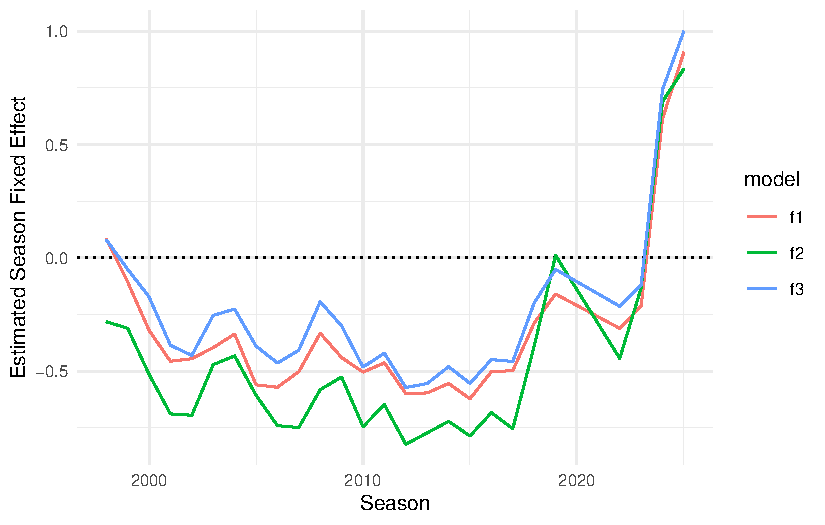
\includegraphics[keepaspectratio]{index_files/figure-pdf/fig-season-coefs2-1.pdf}}

}

\caption{\label{fig-season-coefs2}Estimated season-level fixed effects
for percentage of arena capacity models.}

\end{figure}%

Figure~\ref{fig-season-slopes2} shows that\ldots??

\protect\phantomsection\label{cell-fig-season-slopes2}
\begin{figure}[H]

\centering{

\pandocbounded{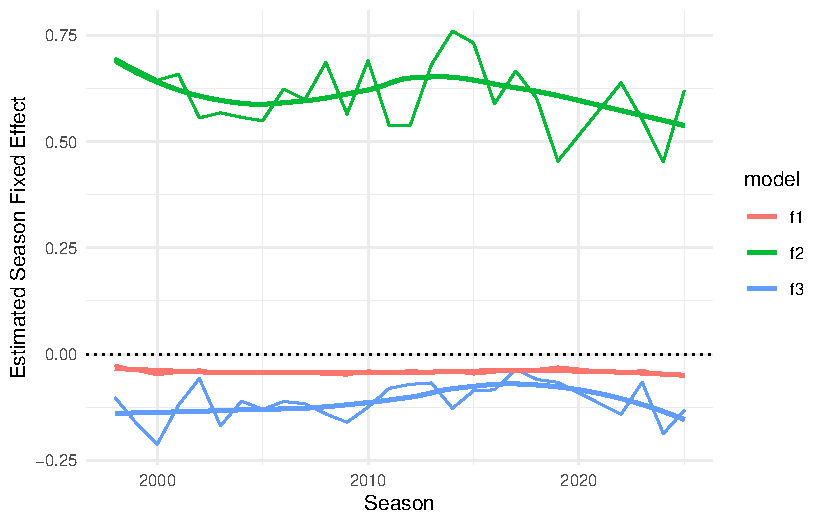
\includegraphics[keepaspectratio]{index_files/figure-pdf/fig-season-slopes2-1.pdf}}

}

\caption{\label{fig-season-slopes2}Estimated season-level changes in
slopes for percentage of arena capacity models.}

\end{figure}%

\section{Conclusion}\label{conclusion}

\subsection{Key results}\label{key-results}

\subsection{Limitations}\label{limitations}

Because the percentage of arena capacity data is right-censored, we
considered a Tobit regression model (McDonald and Moffitt 1980), but our
residuals violated the normality and homoskedasticity conditions. We
also considered fitting a Beta regression model with a logit link
function, and converting the fixed effects for seasons to random
effects, but those models didn't converge.

We also considered fitting a period-based model but ultimately decided
against this approach. Defining periods by hand would require subjective
decisions about the timing of structural breaks and would risk
introducing researcher bias into the analysis.

\subsection{Future work}\label{future-work}

possibly testing different definitions of UOH and Loss Aversion

\section*{References}\label{references}
\addcontentsline{toc}{section}{References}

\protect\phantomsection\label{refs}
\begin{CSLReferences}{1}{1}
\bibitem[\citeproctext]{ref-AghaBerri2023}
Agha, Nola, and David Berri. 2023. {``Demand for Basketball: A
Comparison of the WNBA and NBA.''} \emph{International Journal of Sport
Finance} 18 (1): 35--44.
\url{https://doi.org/10.32731/IJSF/181.022023.03}.

\bibitem[\citeproctext]{ref-CoatesHumphreysZhou2014}
Coates, Dennis, Brad R. Humphreys, and Li Zhou. 2014.
{``Reference-Dependent Preferences, Loss Aversion, and Live Game
Attendance.''} \emph{Economic Inquiry} 52 (3): 959--73.
\url{https://doi.org/10.1111/ecin.12061}.

\bibitem[\citeproctext]{ref-davis2008interaction}
Davis, Michael C. 2008. {``The Interaction Between Baseball Attendance
and Winning Percentage: A VAR Analysis.''} \emph{International Journal
of Sport Finance} 3 (1): 58--73.
\url{https://doi.org/10.1177/155862350800300105}.

\bibitem[\citeproctext]{ref-davis2009analyzing}
Davis, Michael C. 2009. {``Analyzing the Relationship Between Team
Success and MLB Attendance with GARCH Effects.''} \emph{Journal of
Sports Economics} 10 (1): 44--58.
\url{https://doi.org/10.1177/1527002508327387}.

\bibitem[\citeproctext]{ref-delia2020psychological}
Delia, Elizabeth B. 2020. {``The Psychological Meaning of Team Among
Fans of Women's Sport.''} \emph{Journal of Sport Management} 34 (6):
579--90. \url{https://doi.org/10.1123/jsm.2019-0404}.

\bibitem[\citeproctext]{ref-deschriver2002determinants}
DeSchriver, Timothy D, and Paul E Jensen. 2002. {``Determinants of
Spectator Attendance at NCAA Division II Football Contests.''}
\emph{Journal of Sport Management} 16 (4): 311--30.
\url{https://doi.org/10.1123/jsm.16.4.311}.

\bibitem[\citeproctext]{ref-Elo1978}
Elo, A. E. 1978. \emph{The Rating of Chessplayers, Past and Present}.
New York: Arco Publishing.

\bibitem[\citeproctext]{ref-garcia2020betting}
Garcia, Christopher. 2020. {``"Betting on Women": A Feminist Political
Economic Critique of Ideological Sports Narratives Surrounding the
WNBA.''} \emph{The Political Economy of Communication} 8 (1).
\url{https://polecom.org/index.php/polecom/article/view/119}.

\bibitem[\citeproctext]{ref-hutchinson_gilani_2021_wehoop}
Gilani, Saiem, and Geoffery Hutchinson. 2021. {``Wehoop: Access Women's
Basketball Play by Play Data.''} In \emph{CRAN: Contributed Packages}.
The R Foundation. \url{https://doi.org/10.32614/cran.package.wehoop}.

\bibitem[\citeproctext]{ref-guest2018fan}
Guest, Andrew M, and Anne Luijten. 2018. {``Fan Culture and Motivation
in the Context of Successful Women's Professional Team Sports: A
Mixed-Methods Case Study of Portland Thorns Fandom.''} \emph{Sport in
Society} 21 (7): 1013--30.
\url{https://doi.org/10.1080/17430437.2017.1346620}.

\bibitem[\citeproctext]{ref-horowitz2007if}
Horowitz, Ira. 2007. {``If You Play Well They Will Come-and Vice Versa:
Bidirectional Causality in Major-League Baseball.''} \emph{Managerial
and Decision Economics} 28 (2): 93--105.
\url{https://doi.org/10.1002/mde.1308}.

\bibitem[\citeproctext]{ref-kim2023winning}
Kim, Rhino, and Sue Ryung Chang. 2023. {``Winning Back Attendance:
Effects of Winning Performance, Online Search, and the MLB Rule Changes
for More Dynamic Games.''} \emph{Asia Marketing Journal} 25 (3):
148--59. \url{https://doi.org/10.53728/2765-6500.1616}.

\bibitem[\citeproctext]{ref-lemke2010estimating}
Lemke, Robert J, Matthew Leonard, and Kelebogile Tlhokwane. 2010.
{``Estimating Attendance at Major League Baseball Games for the 2007
Season.''} \emph{Journal of Sports Economics} 11 (3): 316--48.
\url{https://doi.org/10.1177/1527002509337212}.

\bibitem[\citeproctext]{ref-leslie2022football}
Leslie-Walker, Anika, and Claire Mulvenna. 2022. {``The Football
Association's Women's Super League and Female Soccer Fans: Fan
Engagement and the Importance of Supporter Clubs.''} \emph{Soccer \&
Society} 23 (3): 314--27.
\url{https://doi.org/10.1080/14660970.2022.2037218}.

\bibitem[\citeproctext]{ref-mackinnon1985some}
MacKinnon, James G, and Halbert White. 1985. {``Some
Heteroskedasticity-Consistent Covariance Matrix Estimators with Improved
Finite Sample Properties.''} \emph{Journal of Econometrics} 29 (3):
305--25. \url{https://doi.org/10.1016/0304-4076(85)90158-7}.

\bibitem[\citeproctext]{ref-mcdonald1980uses}
McDonald, John F, and Robert A Moffitt. 1980. {``The Uses of {Tobit}
Analysis.''} \emph{The Review of Economics and Statistics}, 318--21.
\url{https://www.jstor.org/stable/1924766}.

\bibitem[\citeproctext]{ref-noll1974attendance}
Noll, Roger G. 1974. \emph{Attendance and Price Setting}. Edited by
Roger G Noll. Washington, D.C.: Brookings Institution.

\bibitem[\citeproctext]{ref-papke1996econometric}
Papke, Leslie E, and Jeffrey M Wooldridge. 1996. {``Econometric Methods
for Fractional Response Variables with an Application to 401 (k) Plan
Participation Rates.''} \emph{Journal of Applied Econometrics} 11 (6):
619--32.
\url{https://doi.org/10.1002/(SICI)1099-1255(199611)11:6\%3C619::AID-JAE418\%3E3.0.CO;2-1}.

\bibitem[\citeproctext]{ref-paul2019attendance}
Paul, Rodney, Andrew Weinbach, and Nick Riccardi. 2019. {``Attendance in
the Canadian Hockey League: The Impact of Winning, Fighting, Uncertainty
of Outcome, and Weather on Junior Hockey Attendance.''}
\emph{International Journal of Financial Studies} 7 (1): 12.
\url{https://doi.org/10.3390/ijfs7010012}.

\bibitem[\citeproctext]{ref-PerlineNobleStoldt2018}
Perline, Martin M., Jeffrey S. Noble, and G. Clayton Stoldt. 2018.
{``Competitive Balance in NCAA {`Power Conferences:'} The Case of Men's
and Women's Basketball.''} \emph{The Sport Journal} 21.

\bibitem[\citeproctext]{ref-wasserstein2016asa}
Wasserstein, Ronald L, and Nicole A Lazar. 2016. {``The ASA Statement on
p-Values: Context, Process, and Purpose.''} \emph{The American
Statistician} 70 (2): 129--33.
\url{https://doi.org/10.1080/00031305.2016.1154108}.

\bibitem[\citeproctext]{ref-wasserstein2019moving}
Wasserstein, Ronald L, Allen L Schirm, and Nicole A Lazar. 2019.
{``Moving to a World Beyond {`p\textless{} 0.05'}.''} \emph{The American
Statistician} 73 (sup1): 1--19.
\url{https://doi.org/10.1080/00031305.2019.1583913}.

\bibitem[\citeproctext]{ref-wiseman2003team}
Wiseman, Frederick, and Sangit Chatterjee. 2003. {``Team Payroll and
Team Performance in Major League Baseball: 1985--2002.''}
\emph{Economics Bulletin} 1 (2): 1--10.
\url{https://accessecon.com/pubs/eb/2003/volume1/eb-03a10003a.pdf}.

\bibitem[\citeproctext]{ref-wnba2024recordseason}
WNBA. 2024. {``WNBA Delivers Record‑setting 2024 Season.''}
\url{https://www.wnba.com/news/wnba-delivers-record-setting-2024-season}.

\bibitem[\citeproctext]{ref-woltring2018attendance}
Woltring, Mitchell T. 2018. {``Attendance Still Matters in MLB: The
Relationship with Winning Percentage.''} \emph{The Sport Journal},
November 22.
\url{https://thesportjournal.org/article/attendance-still-matters-in-mlb-the-relationship-with-winning-percentage/}.

\bibitem[\citeproctext]{ref-AcrossTheTimeline}
Zimmerman, Kurtis. 2026. \emph{Game-by-Game Attendance}. Across the
Timeline. \url{https://www.acrossthetimeline.com/wnba/attendance.html}.

\end{CSLReferences}

\section{Appendix}\label{appendix}

\subsection{Distribution of fan
engagement}\label{distribution-of-fan-engagement}

\protect\phantomsection\label{cell-fig-rescaled}
\begin{figure}[H]

\centering{

\pandocbounded{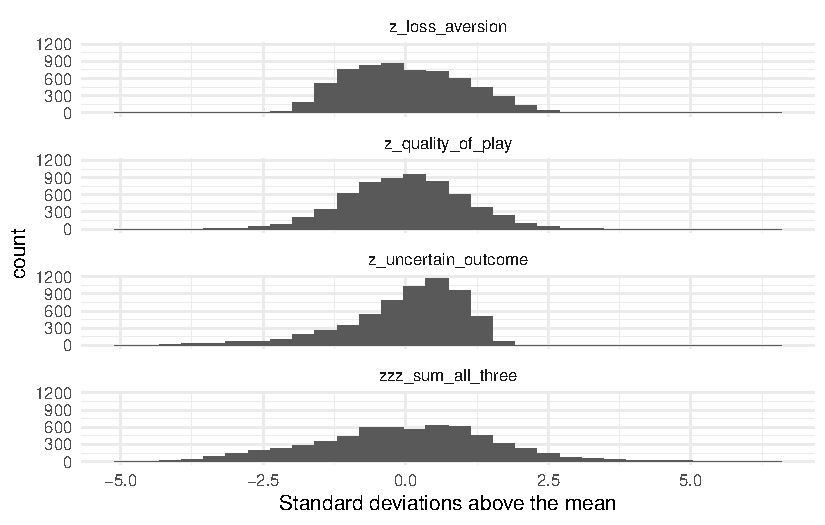
\includegraphics[keepaspectratio]{index_files/figure-pdf/fig-rescaled-1.pdf}}

}

\caption{\label{fig-rescaled}Distribution of fan engagement variables
after rescaling.}

\end{figure}%

\subsection{Relationship between attendance and fan
engagement}\label{relationship-between-attendance-and-fan-engagement}

\protect\phantomsection\label{cell-fig-attend-f1}
\begin{figure}[H]

\centering{

\pandocbounded{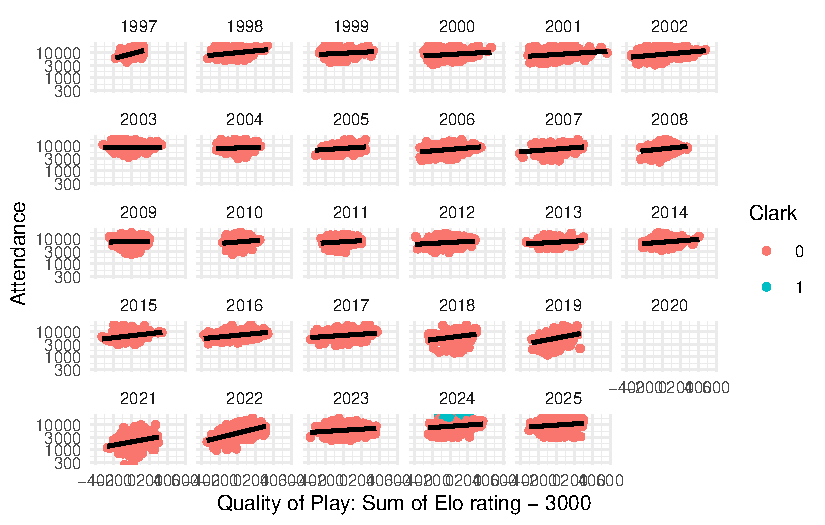
\includegraphics[keepaspectratio]{index_files/figure-pdf/fig-attend-f1-1.pdf}}

}

\caption{\label{fig-attend-f1}WNBA game attendance by season, against
normalized quality of play.}

\end{figure}%

\protect\phantomsection\label{cell-fig-attend-f2}
\begin{figure}[H]

\centering{

\pandocbounded{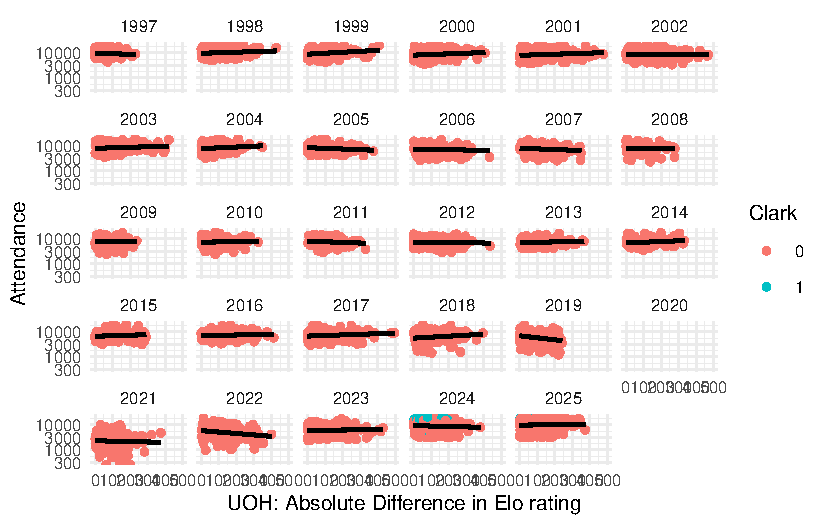
\includegraphics[keepaspectratio]{index_files/figure-pdf/fig-attend-f2-1.pdf}}

}

\caption{\label{fig-attend-f2}WNBA game attendance by season, against
normalized uncertainty of outcome.}

\end{figure}%

\protect\phantomsection\label{cell-fig-capacity-f1}
\begin{figure}[H]

\centering{

\pandocbounded{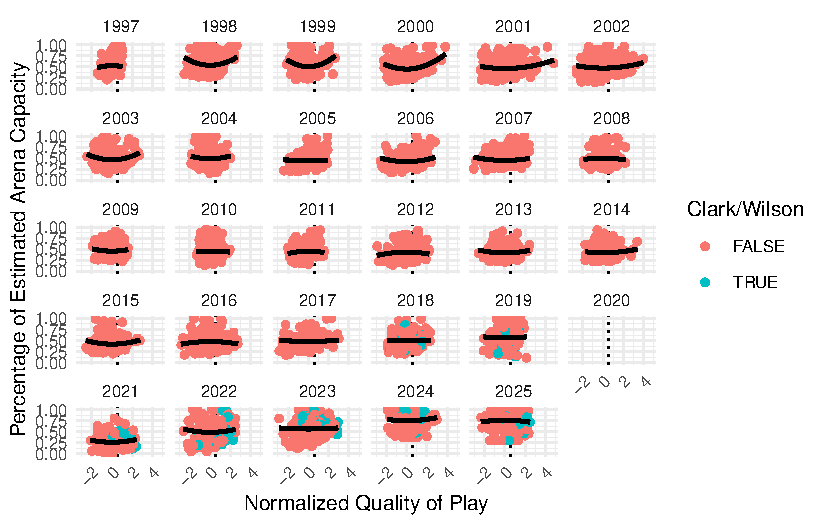
\includegraphics[keepaspectratio]{index_files/figure-pdf/fig-capacity-f1-1.pdf}}

}

\caption{\label{fig-capacity-f1}asd}

\end{figure}%

\protect\phantomsection\label{cell-fig-capacity-f2}
\begin{figure}[H]

\centering{

\pandocbounded{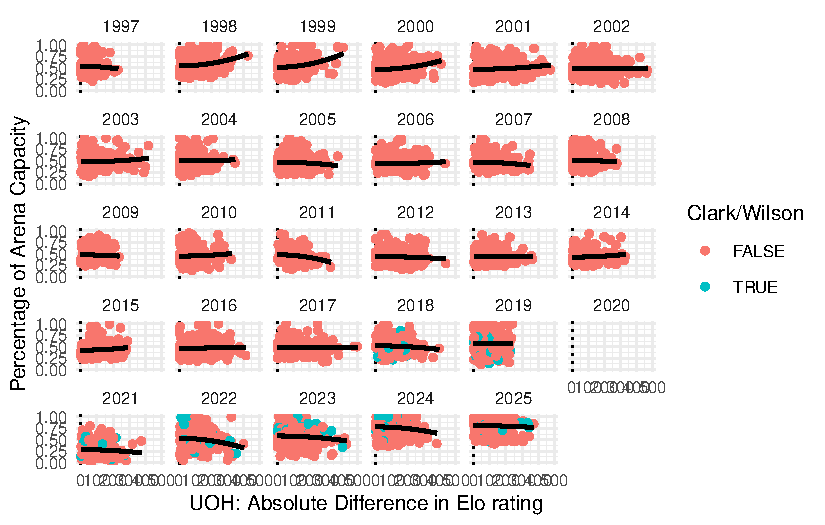
\includegraphics[keepaspectratio]{index_files/figure-pdf/fig-capacity-f2-1.pdf}}

}

\caption{\label{fig-capacity-f2}asd}

\end{figure}%

\subsection{Model fitting metrics for attendance
model}\label{sec-fit-tobit}

{

\begin{longtable}[]{@{}lrrrrr@{}}

\caption{\label{tbl-glance}Model fit}

\tabularnewline

\toprule\noalign{}
model & nobs & df.residual & logLik & AIC & BIC \\
\midrule\noalign{}
\endhead
\bottomrule\noalign{}
\endlastfoot
1 & 5063 & 9991 & -1283.677 & 2837.354 & 3718.865 \\

\end{longtable}

}

{

\begin{longtable}[]{@{}
  >{\raggedright\arraybackslash}p{(\linewidth - 10\tabcolsep) * \real{0.5673}}
  >{\raggedleft\arraybackslash}p{(\linewidth - 10\tabcolsep) * \real{0.0288}}
  >{\raggedleft\arraybackslash}p{(\linewidth - 10\tabcolsep) * \real{0.1538}}
  >{\raggedleft\arraybackslash}p{(\linewidth - 10\tabcolsep) * \real{0.0865}}
  >{\raggedleft\arraybackslash}p{(\linewidth - 10\tabcolsep) * \real{0.0962}}
  >{\raggedleft\arraybackslash}p{(\linewidth - 10\tabcolsep) * \real{0.0673}}@{}}

\caption{\label{tbl-anova-tobit}Analysis of variance for terms in models
for the natural logarithm of attendance.}

\tabularnewline

\toprule\noalign{}
\begin{minipage}[b]{\linewidth}\raggedright
\end{minipage} & \begin{minipage}[b]{\linewidth}\raggedleft
Df
\end{minipage} & \begin{minipage}[b]{\linewidth}\raggedleft
X2 log Lik Diff
\end{minipage} & \begin{minipage}[b]{\linewidth}\raggedleft
Resid Df
\end{minipage} & \begin{minipage}[b]{\linewidth}\raggedleft
Log Lik
\end{minipage} & \begin{minipage}[b]{\linewidth}\raggedleft
Pr Chi
\end{minipage} \\
\midrule\noalign{}
\endhead
\bottomrule\noalign{}
\endlastfoot
I(z1\_quality\_of\_play) & 1 & 210.087 & 10018 & -1474.428 & 0.000 \\
I(z2\_uncertain\_outcome) & 1 & 0.196 & 10018 & -1305.246 & 0.658 \\
I(z3\_loss\_aversion) & 1 & 173.653 & 10018 & -1463.765 & 0.000 \\
factor(name\_current) & 12 & 1026.381 & 10003 & -1796.867 & 0.000 \\
median\_income & 1 & 17.205 & 9992 & -1292.279 & 0.000 \\
metro\_pop & 1 & 6.669 & 9992 & -1287.011 & 0.010 \\
is\_cc & 1 & 245.851 & 9992 & -1406.602 & 0.000 \\
is\_aw & 1 & 3.322 & 9992 & -1285.338 & 0.068 \\
factor(season\_id) & 26 & 774.641 & 10095 & -1869.156 & 0.000 \\
as.character(wday(game\_date, label = TRUE, abbr = FALSE)) & 6 & 179.939
& 9997 & -1373.646 & 0.000 \\
as.character(month(game\_date, label = TRUE, abbr = FALSE)) & 4 &
152.937 & 9995 & -1360.145 & 0.000 \\
I(z1\_quality\_of\_play):factor(season\_id) & 26 & 171.416 & 10017 &
-1369.385 & 0.000 \\
I(z2\_uncertain\_outcome):factor(season\_id) & 26 & 42.942 & 10017 &
-1305.148 & 0.020 \\
I(z3\_loss\_aversion):factor(season\_id) & 26 & 186.524 & 10017 &
-1376.939 & 0.000 \\

\end{longtable}

}

\subsection{Model fitting metrics for percentage of arena capacity
model}\label{sec-fit-papke}

{

\begin{longtable}[]{@{}
  >{\raggedleft\arraybackslash}p{(\linewidth - 14\tabcolsep) * \real{0.1867}}
  >{\raggedleft\arraybackslash}p{(\linewidth - 14\tabcolsep) * \real{0.1067}}
  >{\raggedleft\arraybackslash}p{(\linewidth - 14\tabcolsep) * \real{0.1333}}
  >{\raggedleft\arraybackslash}p{(\linewidth - 14\tabcolsep) * \real{0.1067}}
  >{\raggedleft\arraybackslash}p{(\linewidth - 14\tabcolsep) * \real{0.1200}}
  >{\raggedleft\arraybackslash}p{(\linewidth - 14\tabcolsep) * \real{0.1200}}
  >{\raggedleft\arraybackslash}p{(\linewidth - 14\tabcolsep) * \real{0.1600}}
  >{\raggedleft\arraybackslash}p{(\linewidth - 14\tabcolsep) * \real{0.0667}}@{}}

\caption{\label{tbl-glance2}Comparison of percentage of arena capacity
models.}

\tabularnewline

\toprule\noalign{}
\begin{minipage}[b]{\linewidth}\raggedleft
null.deviance
\end{minipage} & \begin{minipage}[b]{\linewidth}\raggedleft
df.null
\end{minipage} & \begin{minipage}[b]{\linewidth}\raggedleft
logLik
\end{minipage} & \begin{minipage}[b]{\linewidth}\raggedleft
AIC
\end{minipage} & \begin{minipage}[b]{\linewidth}\raggedleft
BIC
\end{minipage} & \begin{minipage}[b]{\linewidth}\raggedleft
deviance
\end{minipage} & \begin{minipage}[b]{\linewidth}\raggedleft
df.residual
\end{minipage} & \begin{minipage}[b]{\linewidth}\raggedleft
nobs
\end{minipage} \\
\midrule\noalign{}
\endhead
\bottomrule\noalign{}
\endlastfoot
841.2874 & 5062 & -2977.425 & 6222.85 & 7097.831 & 473.3406 & 4929 &
5063 \\

\end{longtable}

}

{

\begin{longtable}[]{@{}
  >{\raggedright\arraybackslash}p{(\linewidth - 10\tabcolsep) * \real{0.5413}}
  >{\raggedleft\arraybackslash}p{(\linewidth - 10\tabcolsep) * \real{0.0275}}
  >{\raggedleft\arraybackslash}p{(\linewidth - 10\tabcolsep) * \real{0.0826}}
  >{\raggedleft\arraybackslash}p{(\linewidth - 10\tabcolsep) * \real{0.1101}}
  >{\raggedleft\arraybackslash}p{(\linewidth - 10\tabcolsep) * \real{0.1651}}
  >{\raggedleft\arraybackslash}p{(\linewidth - 10\tabcolsep) * \real{0.0734}}@{}}

\caption{\label{tbl-anova2}Analysis of variance for terms in models for
percentage of arena capacity.}

\tabularnewline

\toprule\noalign{}
\begin{minipage}[b]{\linewidth}\raggedright
Term
\end{minipage} & \begin{minipage}[b]{\linewidth}\raggedleft
Df
\end{minipage} & \begin{minipage}[b]{\linewidth}\raggedleft
Deviance
\end{minipage} & \begin{minipage}[b]{\linewidth}\raggedleft
Df Residual
\end{minipage} & \begin{minipage}[b]{\linewidth}\raggedleft
Residual Deviance
\end{minipage} & \begin{minipage}[b]{\linewidth}\raggedleft
P Value
\end{minipage} \\
\midrule\noalign{}
\endhead
\bottomrule\noalign{}
\endlastfoot
I(z1\_quality\_of\_play) & 1 & 23.076 & 5061 & 818.212 & 0.000 \\
I(z2\_uncertain\_outcome) & 1 & 0.008 & 5060 & 818.203 & 0.927 \\
I(z3\_loss\_aversion) & 1 & 9.976 & 5059 & 808.227 & 0.002 \\
factor(name\_current) & 12 & 97.666 & 5047 & 710.561 & 0.000 \\
median\_income & 1 & 80.763 & 5046 & 629.798 & 0.000 \\
metro\_pop & 1 & 2.846 & 5045 & 626.952 & 0.092 \\
is\_cc & 1 & 33.209 & 5044 & 593.743 & 0.000 \\
is\_aw & 1 & 3.128 & 5043 & 590.615 & 0.077 \\
factor(season\_id) & 26 & 69.636 & 5017 & 520.980 & 0.000 \\
as.character(wday(game\_date, label = TRUE, abbr = FALSE)) & 6 & 15.048
& 5011 & 505.932 & 0.020 \\
as.character(month(game\_date, label = TRUE, abbr = FALSE)) & 4 & 12.826
& 5007 & 493.106 & 0.012 \\
I(z1\_quality\_of\_play):factor(season\_id) & 26 & 5.860 & 4981 &
487.246 & 1.000 \\
I(z2\_uncertain\_outcome):factor(season\_id) & 26 & 3.613 & 4955 &
483.632 & 1.000 \\
I(z3\_loss\_aversion):factor(season\_id) & 26 & 10.292 & 4929 & 473.341
& 0.997 \\

\end{longtable}

}




\end{document}
